目標値変更のシミュレーションによって制御器に関する各パラメータの有効な値を決定する。 シミュレーションにはJAMOXを用いた。
% --------------------------------------------------------------------------------------
\section{重み行列の変更による制御性能評価}
	LQ最適制御に基づく状態フィードバック$F$を設計するために
	連続時間線形二次レギュレーターを用いる。この時、連続時間線形二次レギュレーターには
	システム行列$A$と入力行列$B$と重み行列$Q,R$が必要である。
	重み行列は、(\ref{eq:Feq3})式で与え、この重み行列を
	調整することで倒立振子の安定化制御の性能を高めることができる。
	そこで、シミュレーションを用いて重み行列を変更させたときの制御性能について考察していき、
	どのような重み行列を用いればよいか決定する。
	\par
	今回は行列$R$の値は変更しないので、行列$Q$のみ値を変更してシミュレーション結果を考察する。
	便宜上、重み行列$Q$の対角成分を左から第1成分、第2成分、第3成分、第4成分と呼ぶことにする。
	以下にシミュレーションを行った各パターンのパラメータをまとめた表とその時のシミュレーション結果を示す。
	\begin{table}[htb]
		\begin{center}
			\caption{重み行列の変更パターン}
			%\medskip
			\begin{tabular}{|c|c|c|c|}\hline
				& 重み行列$Q$ & オブザーバの極$P$ & サンプリング周期$\Delta[\rm{s}]$ \\ \hline\hline
				パターン1 & $Q_1$:$\rm{diag}(1E5,1E5,1,1)$ & $P_1$:$((-60,0),(-60,0))^{'}$ & $\Delta_1$:0.005 \\ \hline
				パターン2 & $Q_2$:$\rm{diag}(1E6,1E5,1,1)$ & $P_1$:$((-60,0),(-60,0))^{'}$ & $\Delta_1$:0.005 \\ \hline
				パターン3 & $Q_3$:$\rm{diag}(1E5,1E6,1,1)$ & $P_1$:$((-60,0),(-60,0))^{'}$ & $\Delta_1$:0.005 \\ \hline
			\end{tabular}
		\end{center}
		\label{table:QRF}
	\end{table}
	
	\begin{figure}[H]
		\centering
		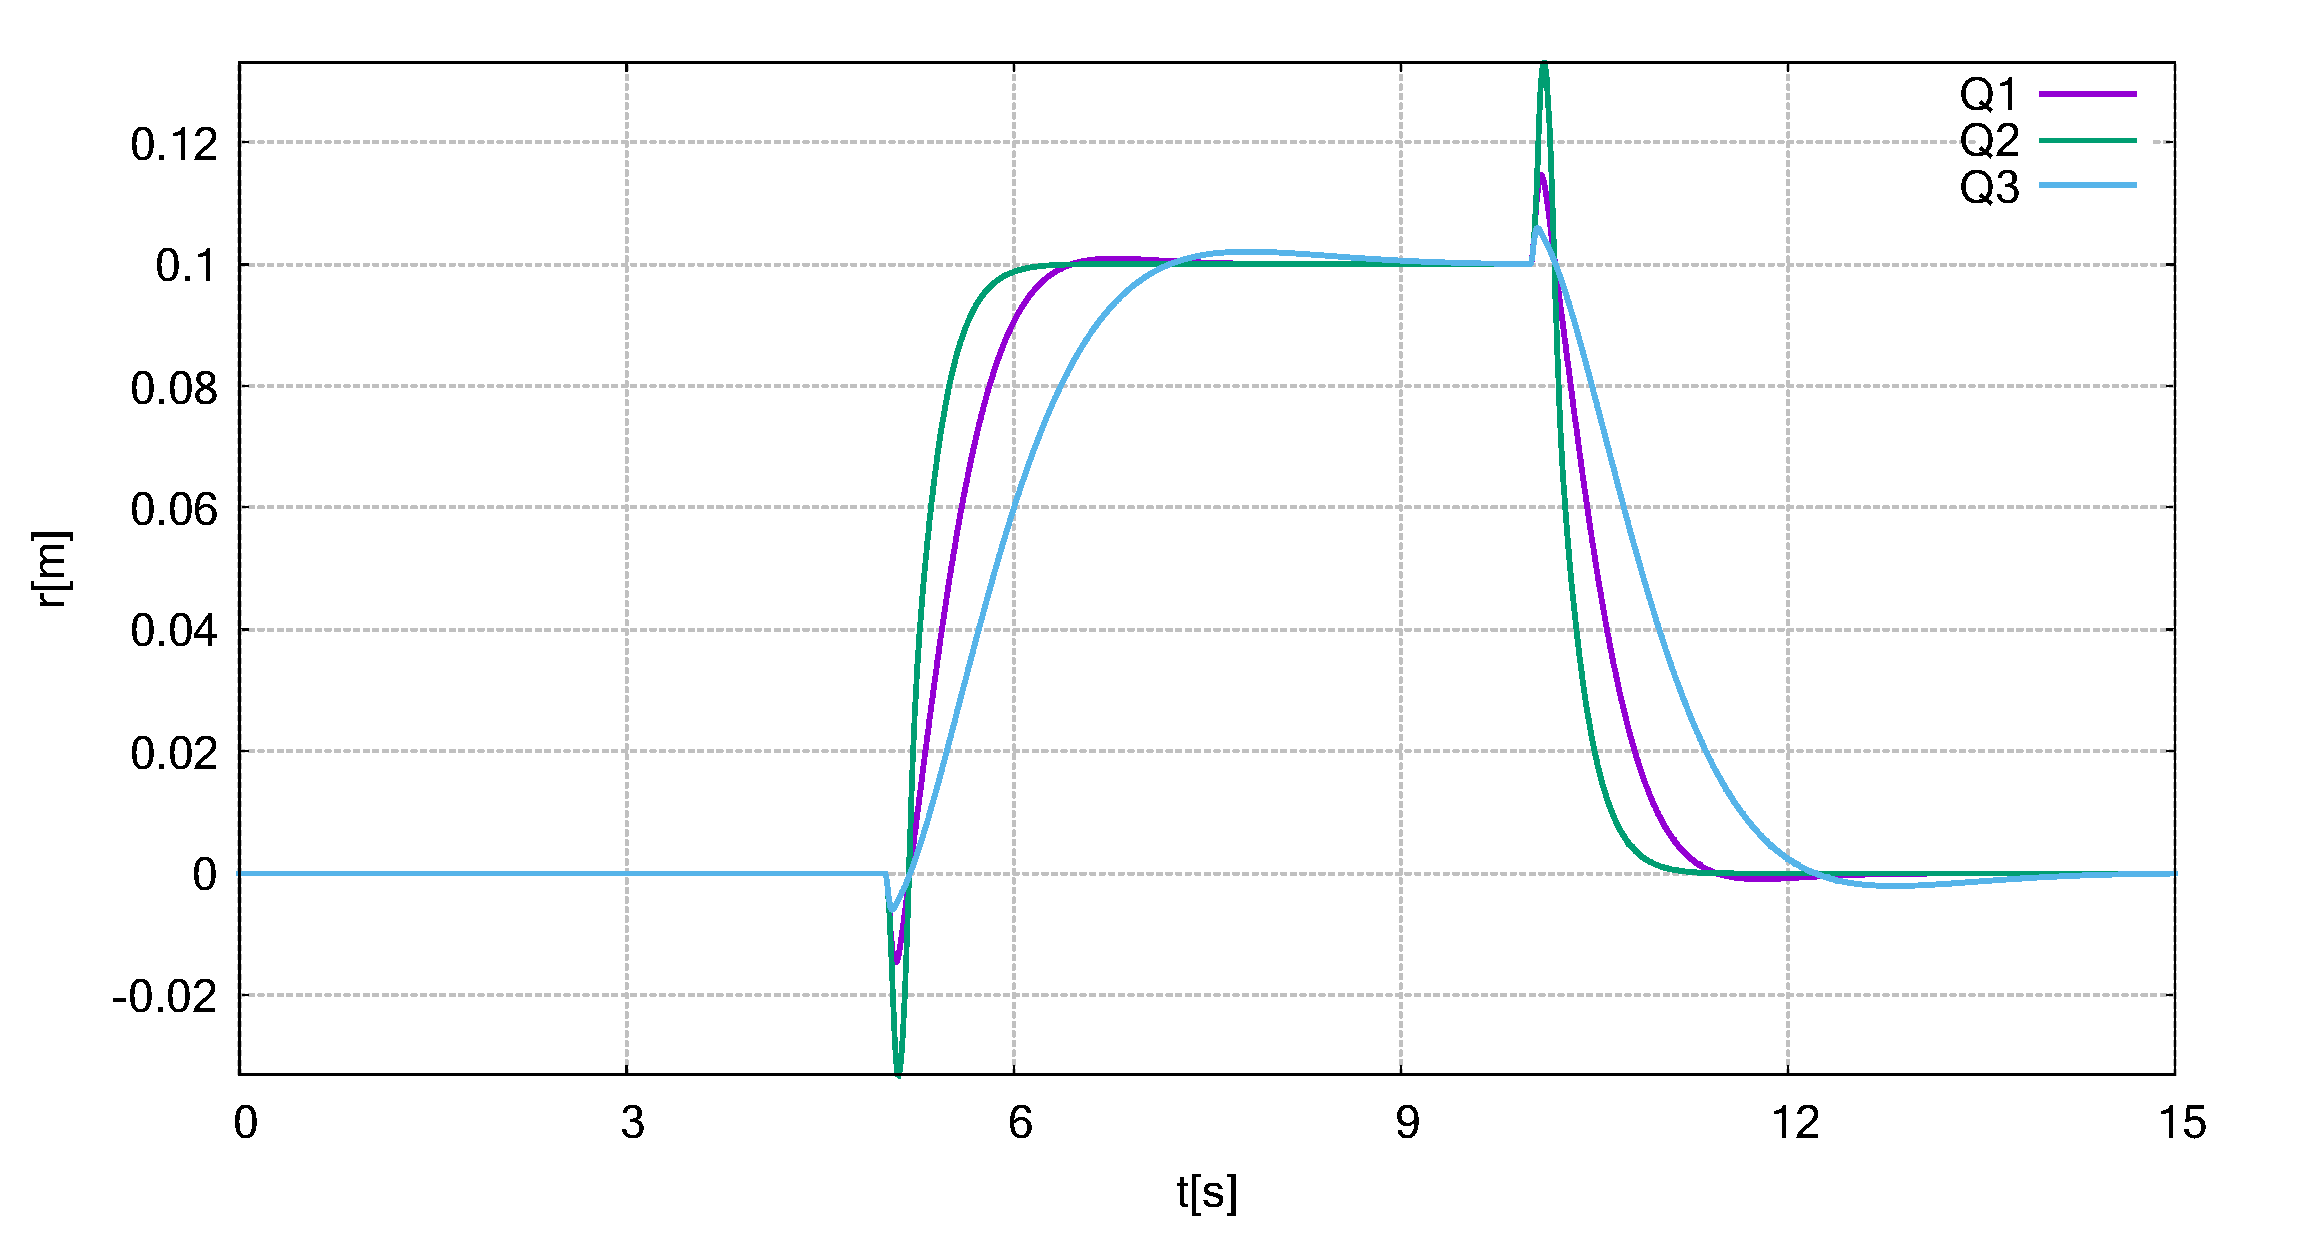
\includegraphics[width=0.8\linewidth]{gazo/simulation_QRF_compare_R.eps}
		\caption{重み行列での比較結果(台車位置)}
		\label{image:simulation_QRF_r}
	\end{figure}
	\begin{figure}[H]
		\centering
		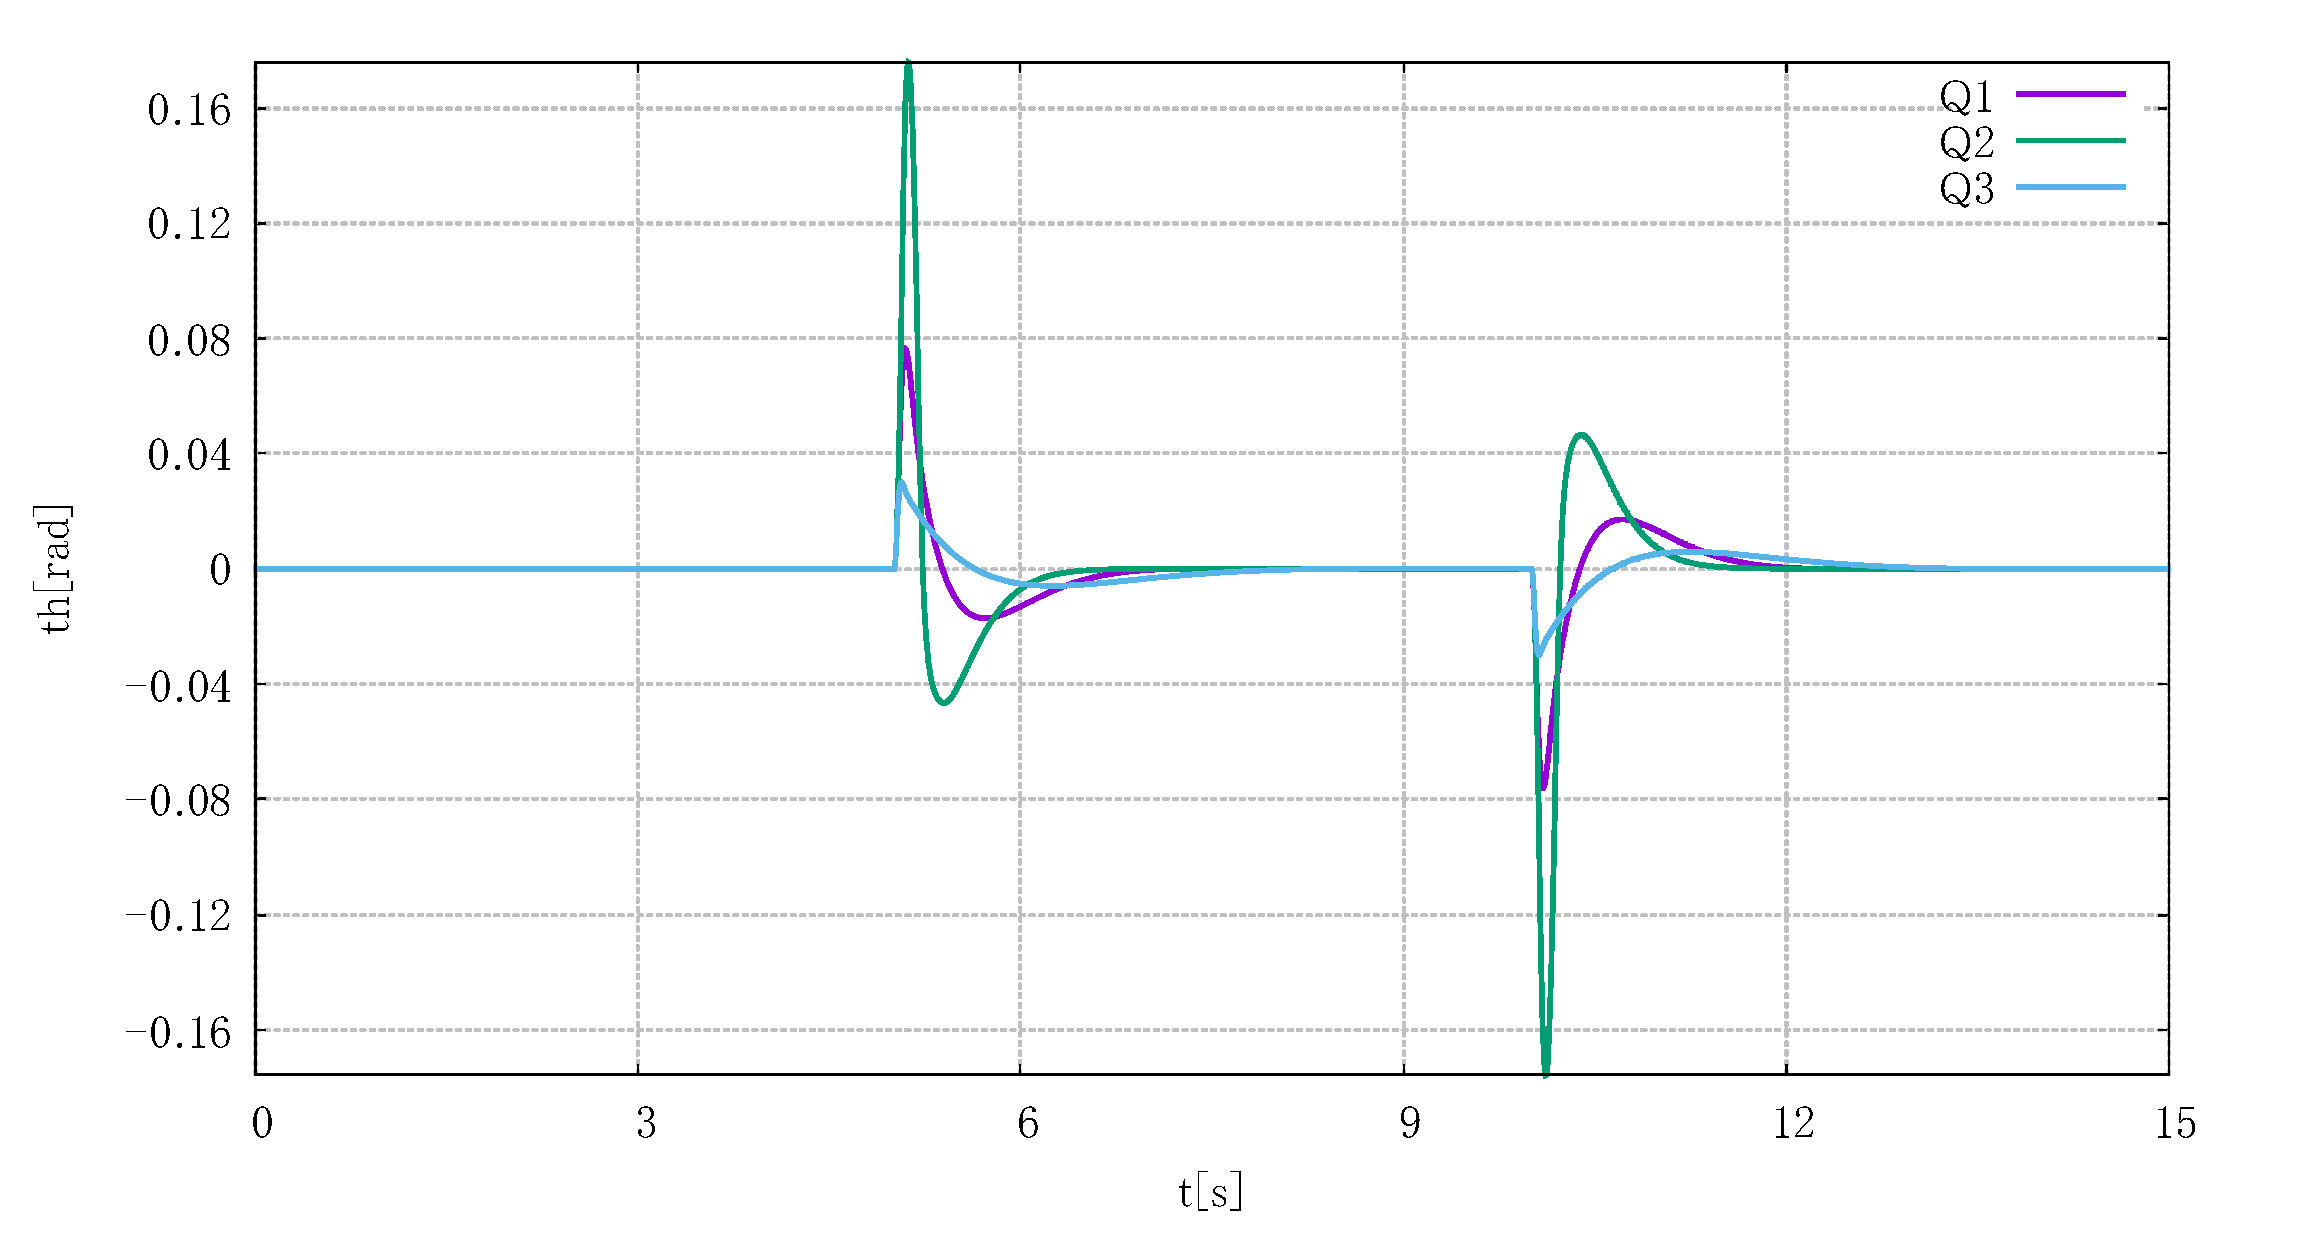
\includegraphics[width=0.8\linewidth]{gazo/simulation_QRF_compare_THETA.eps}
		\caption{重み行列での比較結果(振子角度)}
		\label{image:simulation_QRF_th}
	\end{figure}
	%図のほう要確認
	図(\ref{image:simulation_QRF_r})より$Q_2$の応答が一番早く、$Q_3$の応答が一番遅いことが確認できる。このことから台車の位置$r$の応答をよくするには
	重み行列$Q$の第1成分を大きくすればよいとわかる。また、$Q_1$と$Q_3$の第1成分は同じであるのにもかかわらず、$Q_1$の方が応答が早いことが確認できる。これは
	振子の角度$\theta$の応答をよくする第2成分を大きくした分、バランスが第2成分のほうに偏ってしまい、台車の位置の応答が悪くなったといえる。
	\par
	図(\ref{image:simulation_QRF_th})より、振子の角度についても同じことが言え、第2成分を大きくしている$Q_3$の応答が一番よく、$Q_2$の応答が一番悪い結果となっている。
	\par
	以上から重み行列の調整については以下のことが言える。
	\begin{itemize}
	  \item 重み行列$Q$の各成分は$r,\theta,\dot{r},\dot{\theta}$に対応している
	  \item 応答をよくしたい状態があれば、その状態に対応する成分の値を大きくすればよい
	  \item その場合、大きくした成分に対応する状態にバランスが偏る(つまり、ほかの状態の応答が悪くなる)
	\end{itemize}
	これらを考慮して重み行列を決定すれよい。
	
	
% --------------------------------------------------------------------------------------
\section{オブザーバの極の変更による制御性能評価}
	前章で述べたように、最小次元オブザーバを設計するためにゴピナスの方法を用いる。
	この時、システム行列$A$、入力行列$B$、出力行列$C$、オブザーバの極$P$が必要である。
	オブザーバの極$P$を調整することで倒立振子の安定化制御の応答をよくすることができる。
	同様にシミュレーションによって制御性能を考察していき、適当なオブザーバの極$P$を決定する。
	\par
	1つ考慮しなければならないのは、オブザーバの極と
	閉ループ系の極(つまり、$(A-BF)$の固有値)との位置関係である。
	閉ループ系の極のうち虚軸に最も近い極を$\lambda_{\max}$としたとき、オブザーバーの極$P$は
	\[
		\rm{Re}(P) <5\rm{Re}(\lambda_{max})
	\]
	を考慮して設定する必要がある。
	表(\ref{table:QRF})の$Q_2$を用いて設計した状態フィードバック$F$における閉ループ系の極は
	\begin{equation}
		D=\left[
		\begin{array}{c}
			-0.08\\
			-6.3+1.3i\\
			-6.3+1.3i\\
			-13\\
		\end{array}
		\right]
		\label{eq:Aeig}
	\end{equation}
	である。この中で一番虚軸に近い極は$-0.08$である。よって、少なくともオブザーバーの極$P$は$-0.4$
	より小さい値をとればよいとわかる。
	\par
	以下にシミュレーションを行った各パターンのパラメータをまとめた表とその時のシミュレーション結果を示す。
	\begin{table}[htb]
		\begin{center}
			\caption{オブザーバの極の変更パターン}
			\medskip
			
			\begin{tabular}{|c|c|c|c|}\hline
				\ \ & 重み行列$Q$ & オブザーバの極$P$ & サンプリング周期$\Delta[\rm{s}]$ \\ \hline\hline
				パターン1 & $Q_1$:$\rm{diag}(1E5,1E5,1,1)$ & $P_1$:$((-60,0),(-60,0))^{'}$ & $\Delta_1$:0.005 \\ \hline
				パターン2 & $Q_1$:$\rm{diag}(1E5,1E5,1,1)$ & $P_2$:$((-30,0),(-30,0))^{'}$ & $\Delta_1$:0.005 \\ \hline
			\end{tabular}
		\end{center}
		\label{table:obsP}
	\end{table}
	
	\begin{figure}[H]
		\centering
		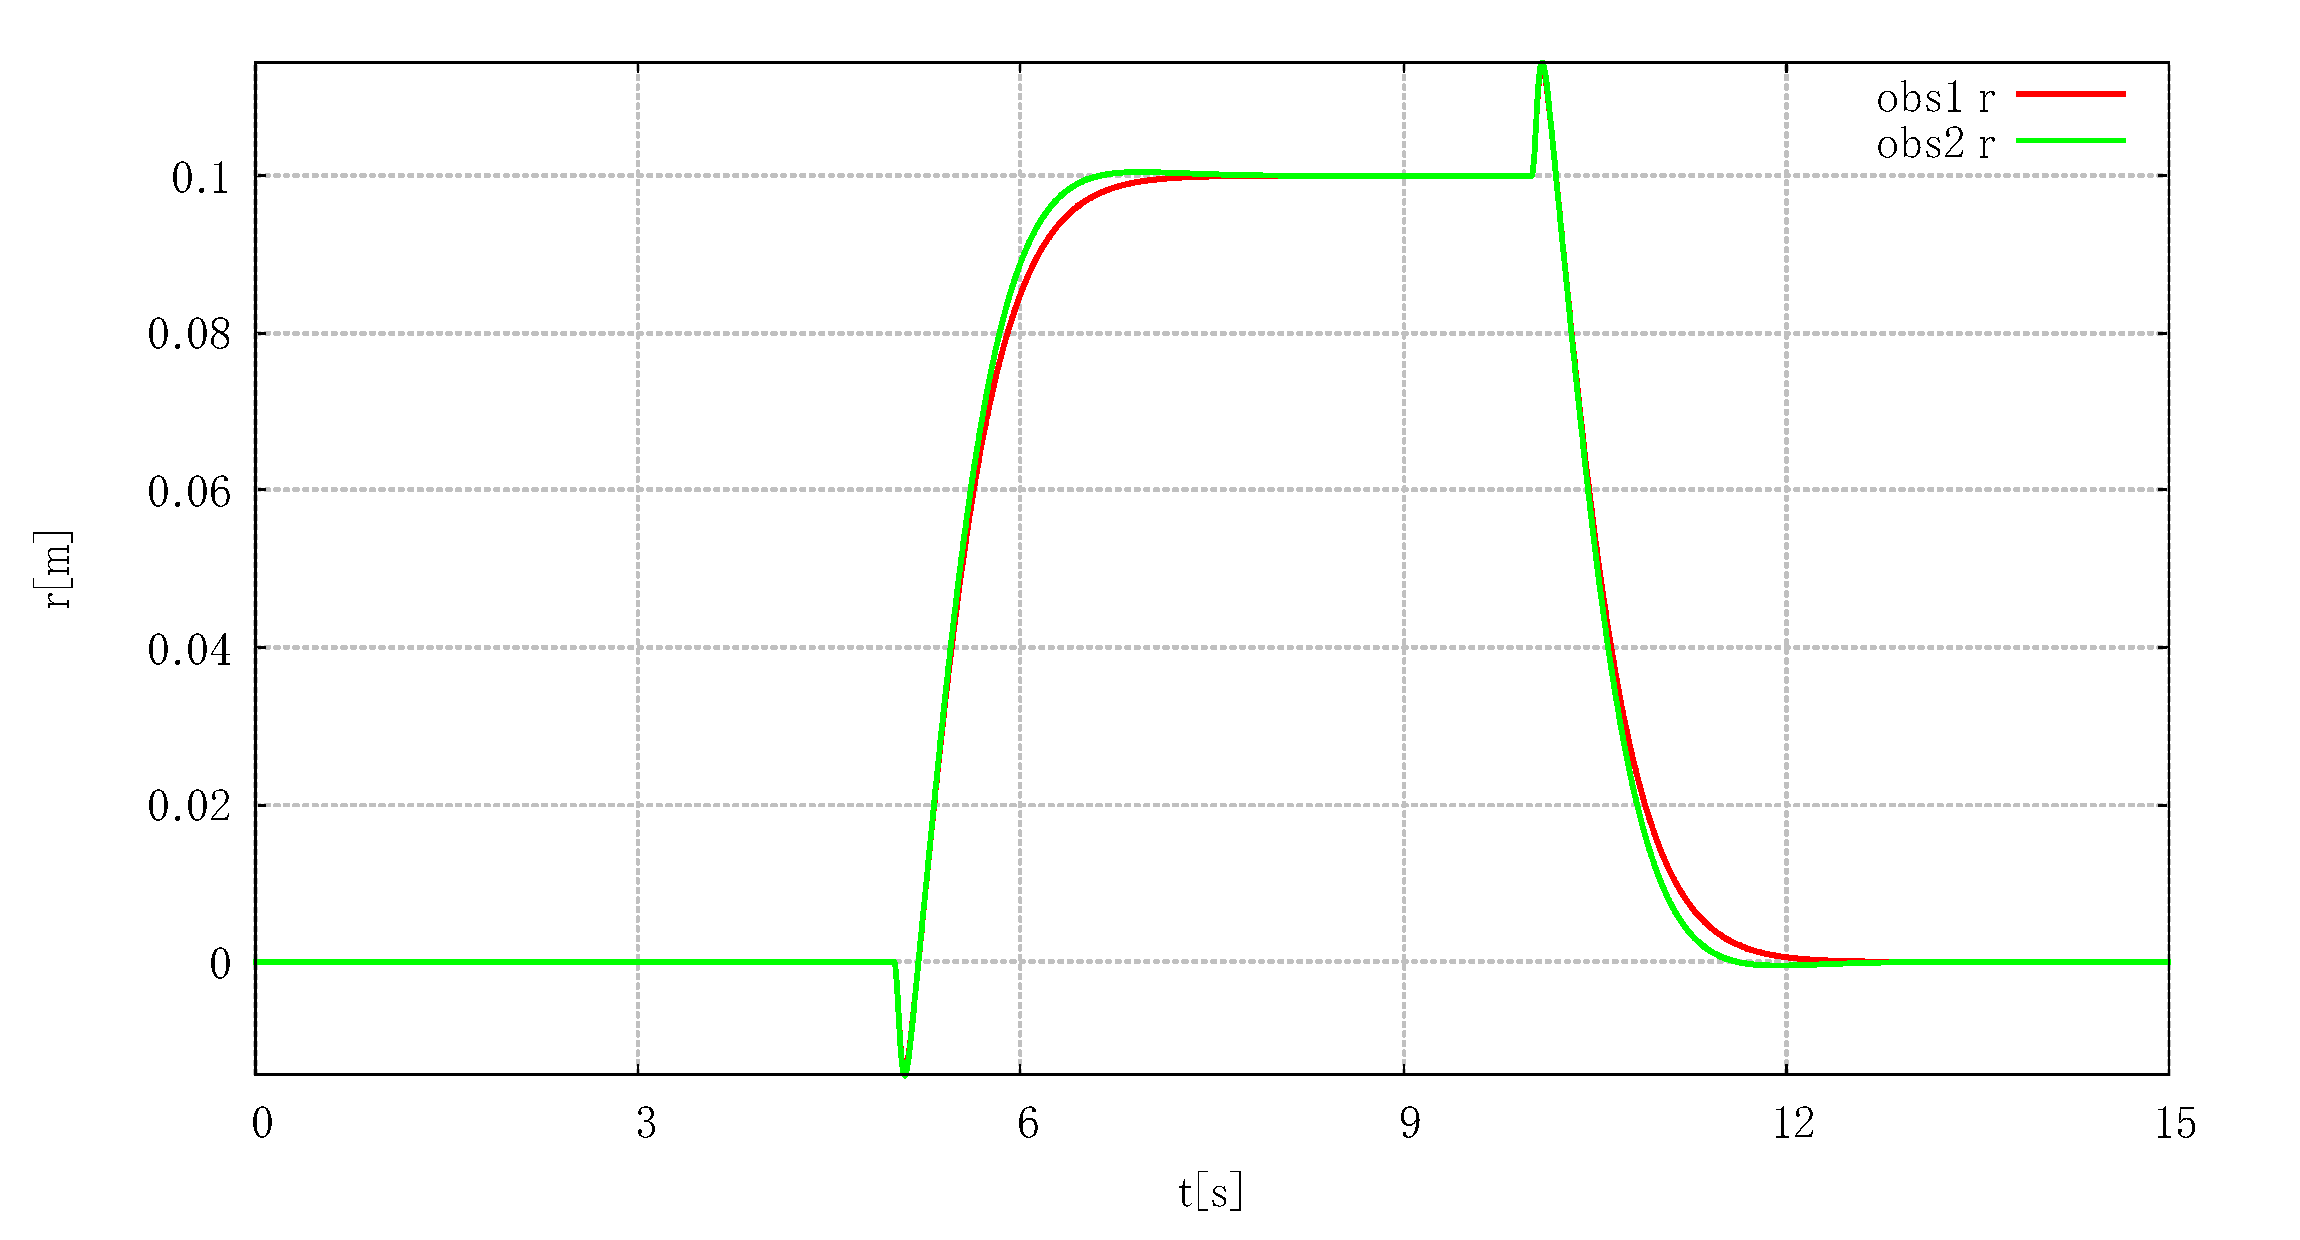
\includegraphics[width=0.8\linewidth]{gazo/simulation_obs_compare_R.eps}
		\caption{オブザーバーの極での比較結果(台車位置)}
		\label{image:simulation_obs_r}
	\end{figure}
	\begin{figure}[H]
		\centering
		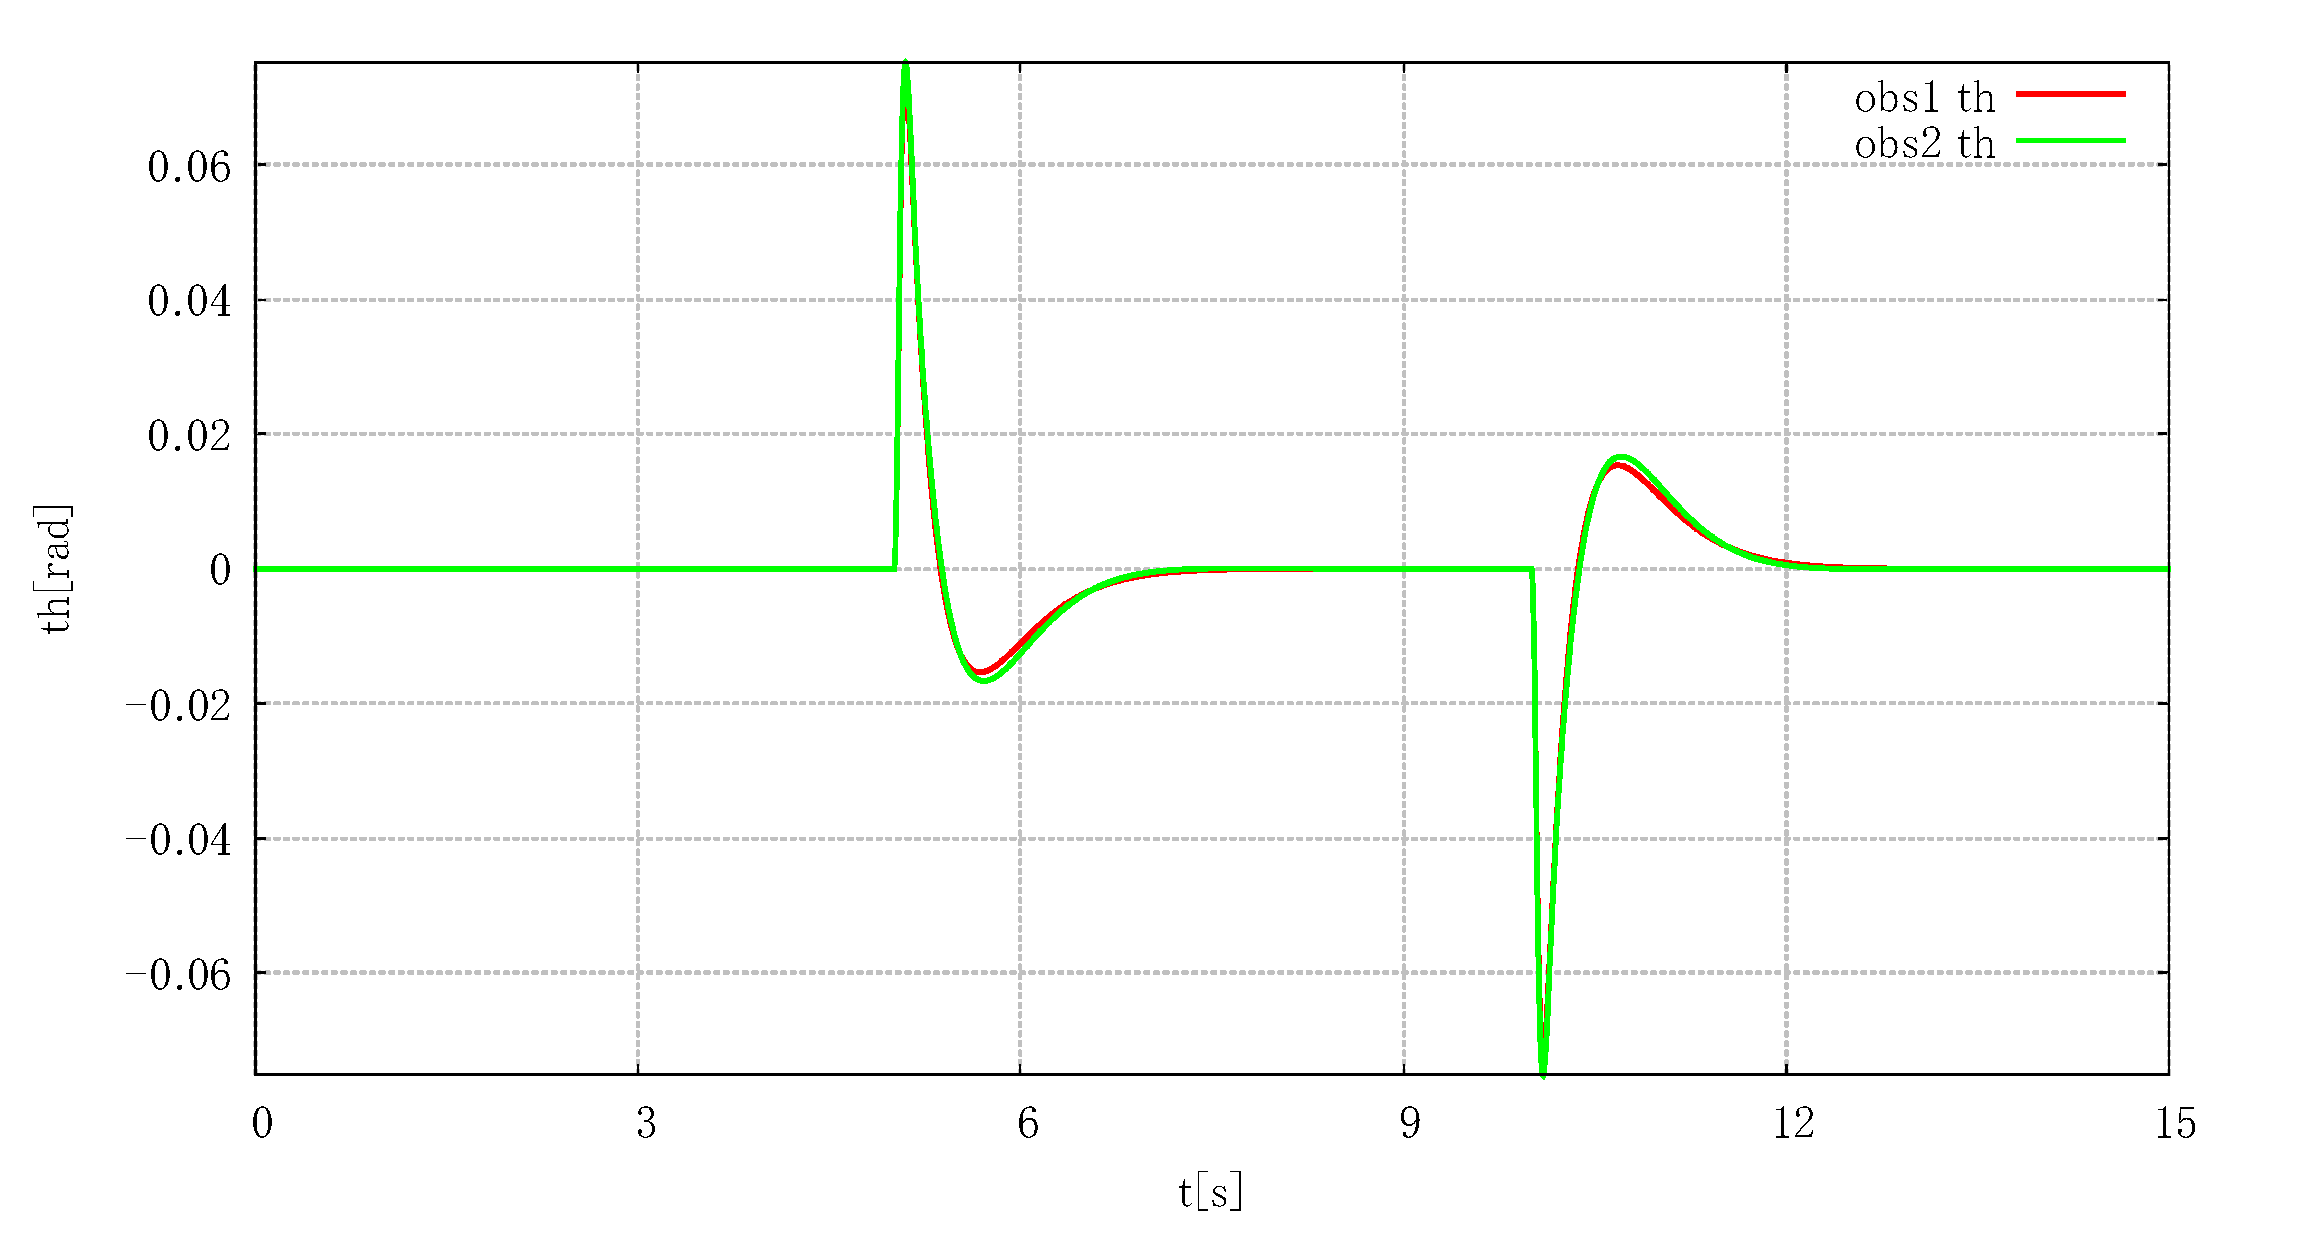
\includegraphics[width=0.8\linewidth]{gazo/simulation_obs_compare_THETA.eps}
		\caption{オブザーバーの極での比較結果(振子角度)}
		\label{image:simulation_obs_theta}
	\end{figure} 
	図\ref{image:simulation_obs_r}と図\ref{image:simulation_obs_theta}からオブザーバの極の違いによる応答の大きな違いは確認できない。
	ここで、倒立振子の状態$x$(台車の速度と振り子の角速度)とオブザーバで推定した値$\hat{x}$(台車の速度と振り子の角速度)
	との差である推定誤差($x-\hat{x}$)の応答波形からオブザーバの極の違いによる考察をする。
	以下に台車の速度と振り子の角速度の推定誤差の図を示す。
	\begin{figure}[H]
		\centering
		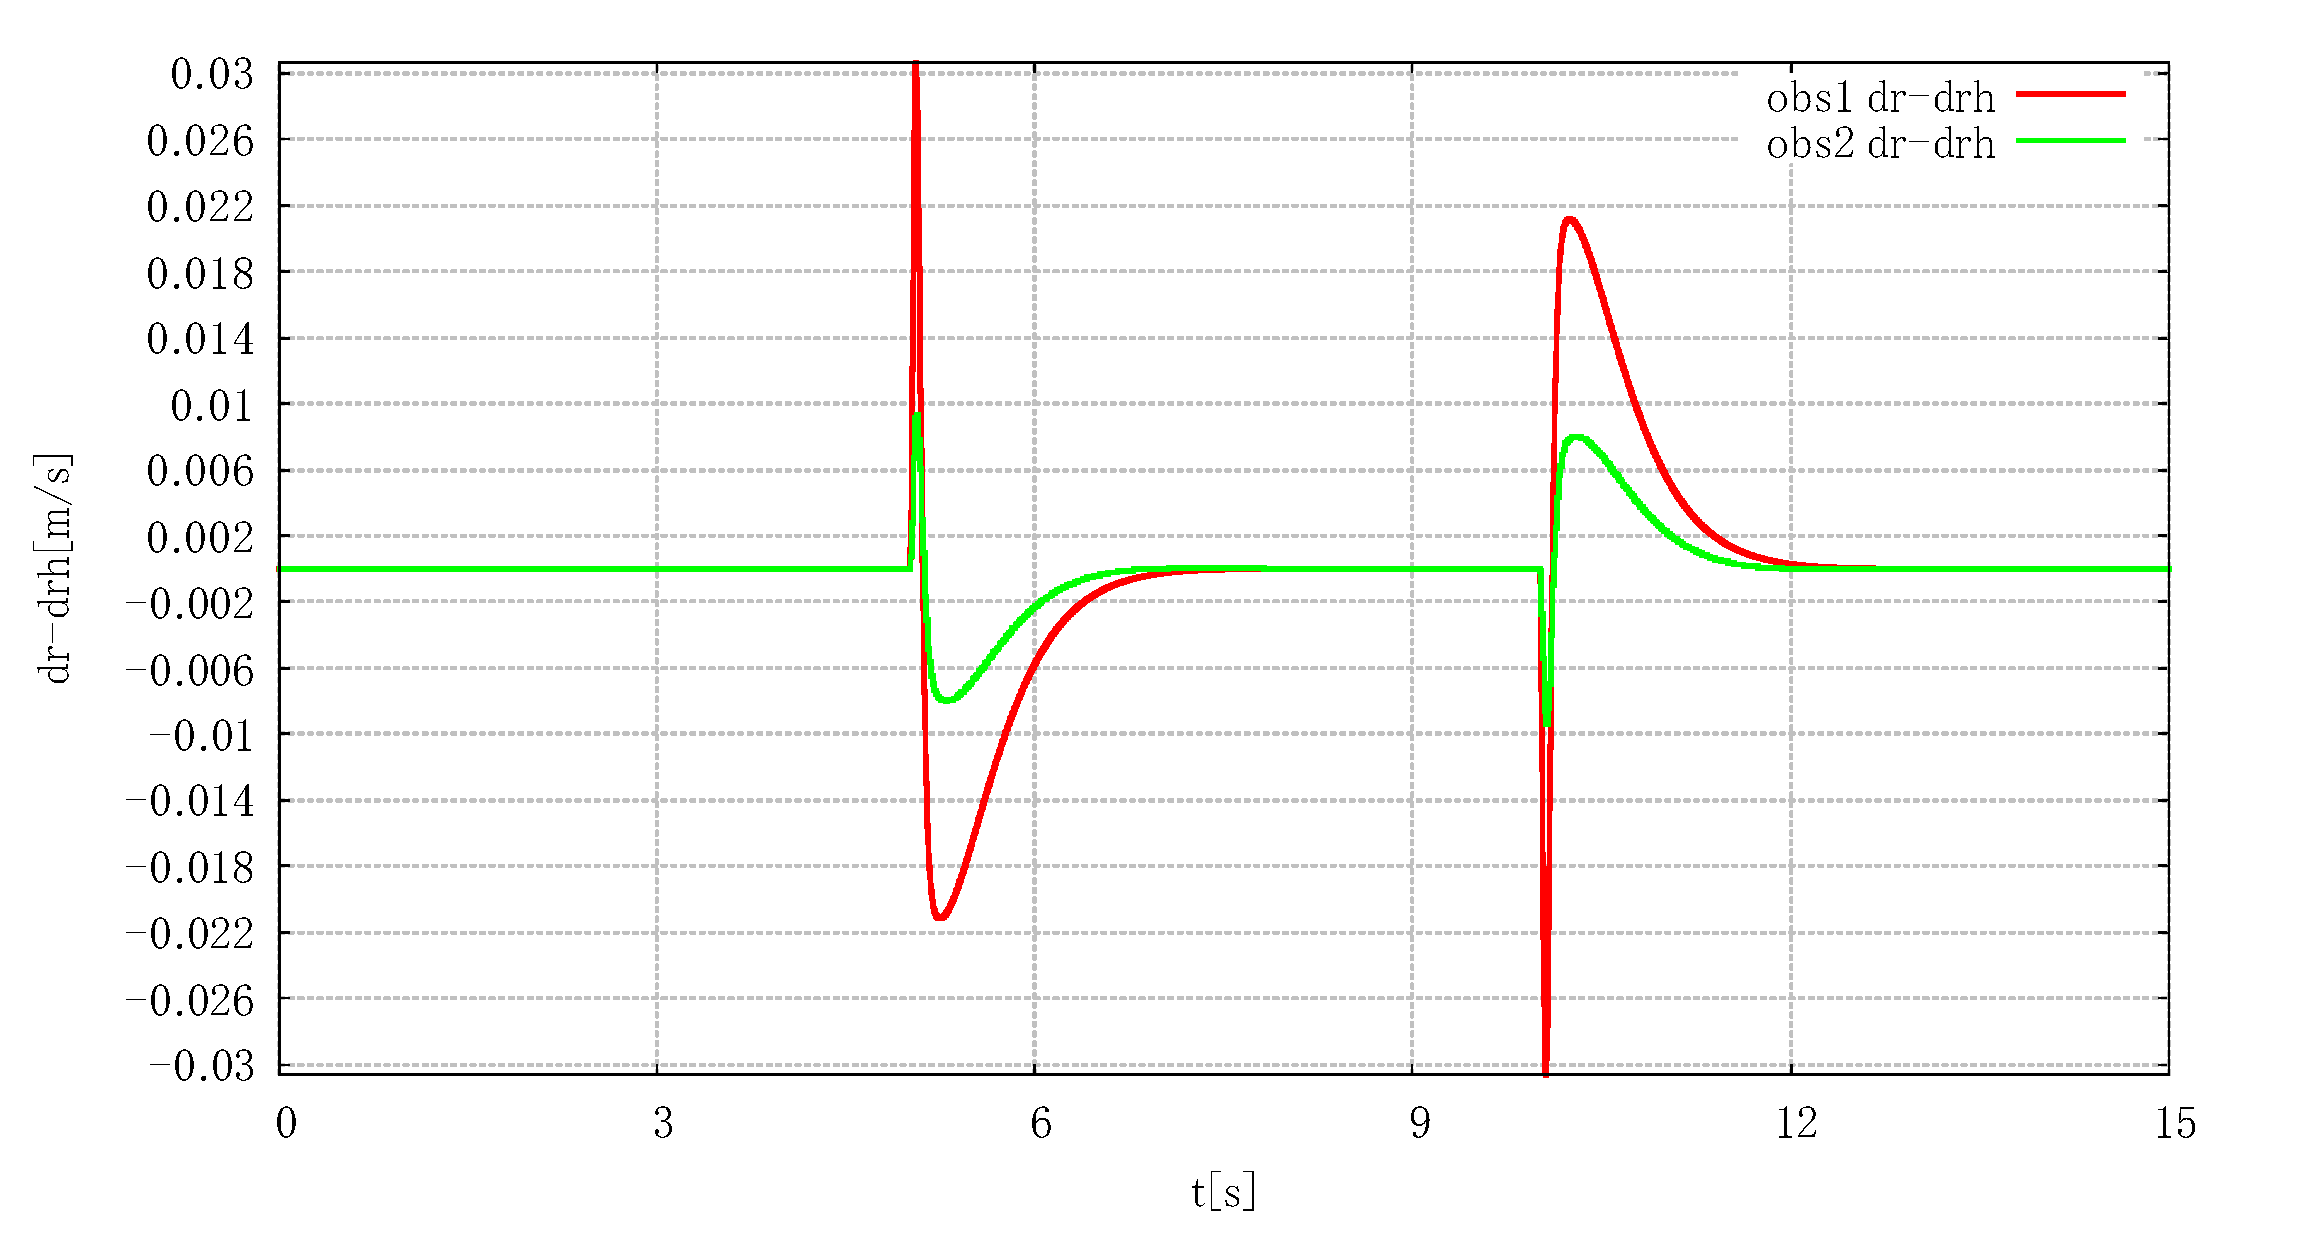
\includegraphics[width=0.8\linewidth]{gazo/simulation_obs_compare_RminusRH.eps}
		\caption{オブザーバーの極での推定誤差の比較(台車の速度)}
		\label{image:simulation_obs_rminusrh}
	\end{figure}
	\begin{figure}[H]
		\centering
		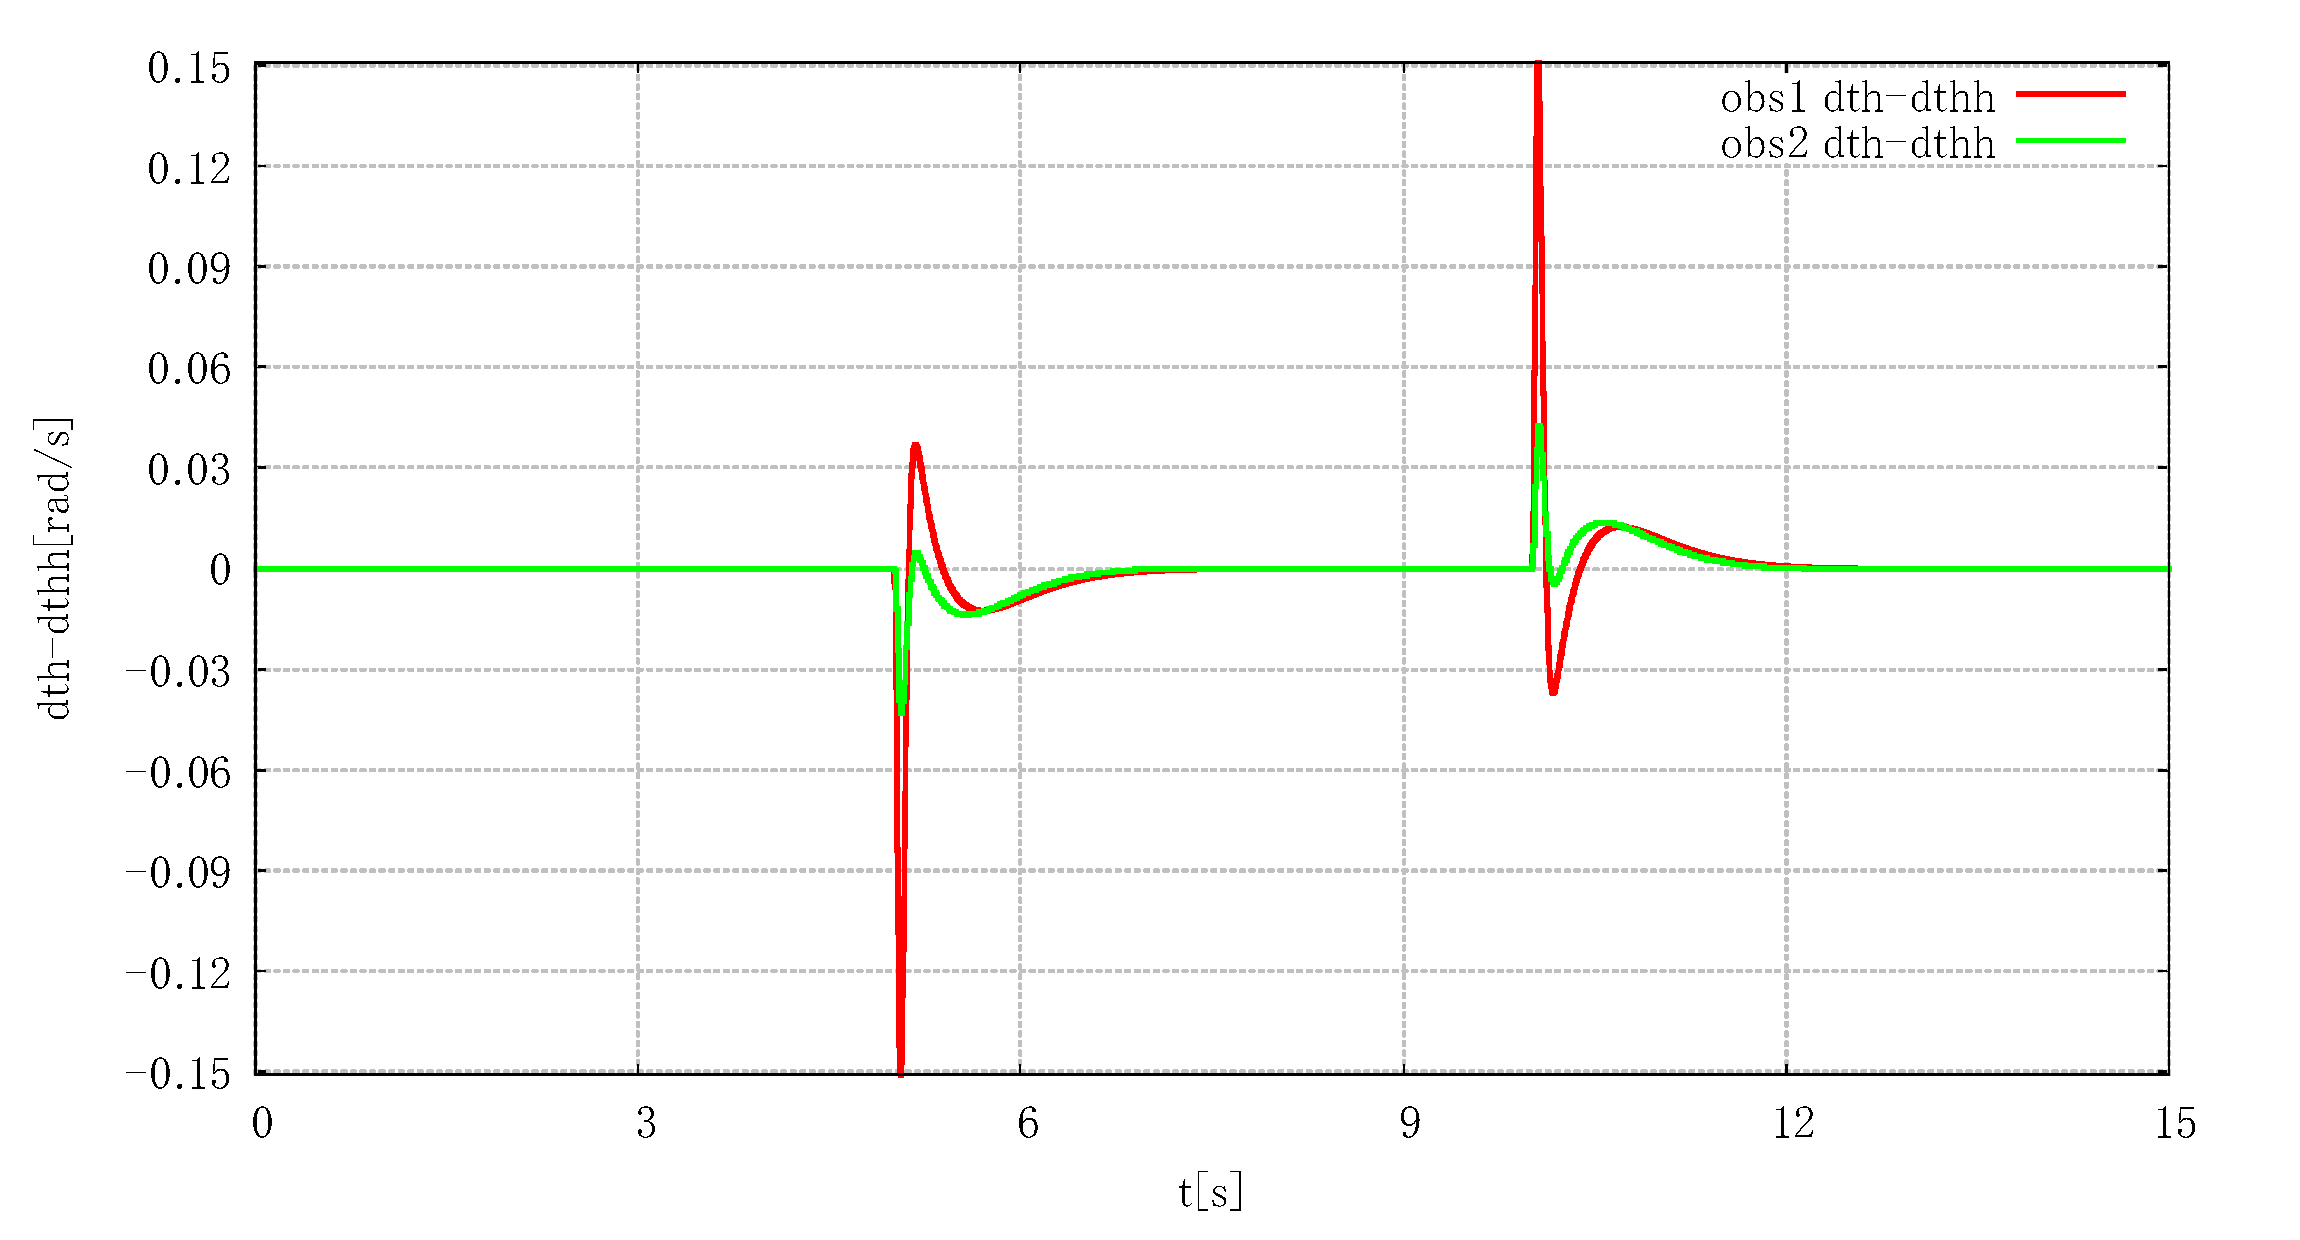
\includegraphics[width=0.8\linewidth]{gazo/simulation_obs_compare_THETAminusTHETAH.eps}
		\caption{オブザーバーの極での推定誤差の比較(振子の角速度)}
		\label{image:simulation_obs_thetaminusthetah}
	\end{figure} 
	図\ref{image:simulation_obs_rminusrh}と図\ref{image:simulation_obs_thetaminusthetah}よりオブザーバの極が
	虚軸から遠いパターン1のほうが推定誤差の収束が若干遅いことがわかる。また、その大きさもパターン1のほうが大きいこともわかる。
	\par
	以上からオブザーバの極配置の調整については以下のことが言える。
	\begin{itemize}
	  \item オブザーバの極は虚軸に近いほうが推定誤差が小さくなり応答はよくなるといえる。
	  \item ただし、閉ループ系の極との位置関係を考慮する必要がある。
	\end{itemize}
	これらを満たすオブザーバの極を決定すればよい。
	
%--------------------------------------------------------------------------------------
\section{サンプリング周期の変更による制御性能評価}
	離散化を行うサンプリング周期$\Delta$を調整することで倒立振子の安定化制御の性能を高めることができる。
	同様にシミュレーションによって制御性能を考察していき、どのようなサンプリング周期をとればよいか決定する。
	ただし、サンプリング周期が短すぎると実験で用いる倒立振子系においてシステム全体がハングアップする恐れ
	があるため、そのような値においてはシミュレーションを行わない。
	\par
	以下にシミュレーションを行った各パターンのパラメータをまとめた表とその時のシミュレーション結果を示す。
	\begin{table}[htb]
		\begin{center}
			\caption{サンプリング周期の変更パターン}
			\medskip
			
			\begin{tabular}{|c|c|c|c|}\hline
				& 重み行列$Q$ & オブザーバの極$P$ & サンプリング周期$\Delta[\rm{s}]$ \\ \hline\hline
				パターン1 & $Q_1$:$\rm{diag}(1E5,1E5,1,1)$ & $P_1$:$((-60,0),(-60,0))^{'}$ & $\Delta_1$:0.005 \\ \hline
				パターン2 & $Q_1$:$\rm{diag}(1E5,1E5,1,1)$ & $P_1$:$((-60,0),(-60,0))^{'}$ & $\Delta_2$:0.01 \\ \hline
			\end{tabular}
		\end{center}
		\label{table:dt}
	\end{table}
	
	\begin{figure}[H]
		\centering
		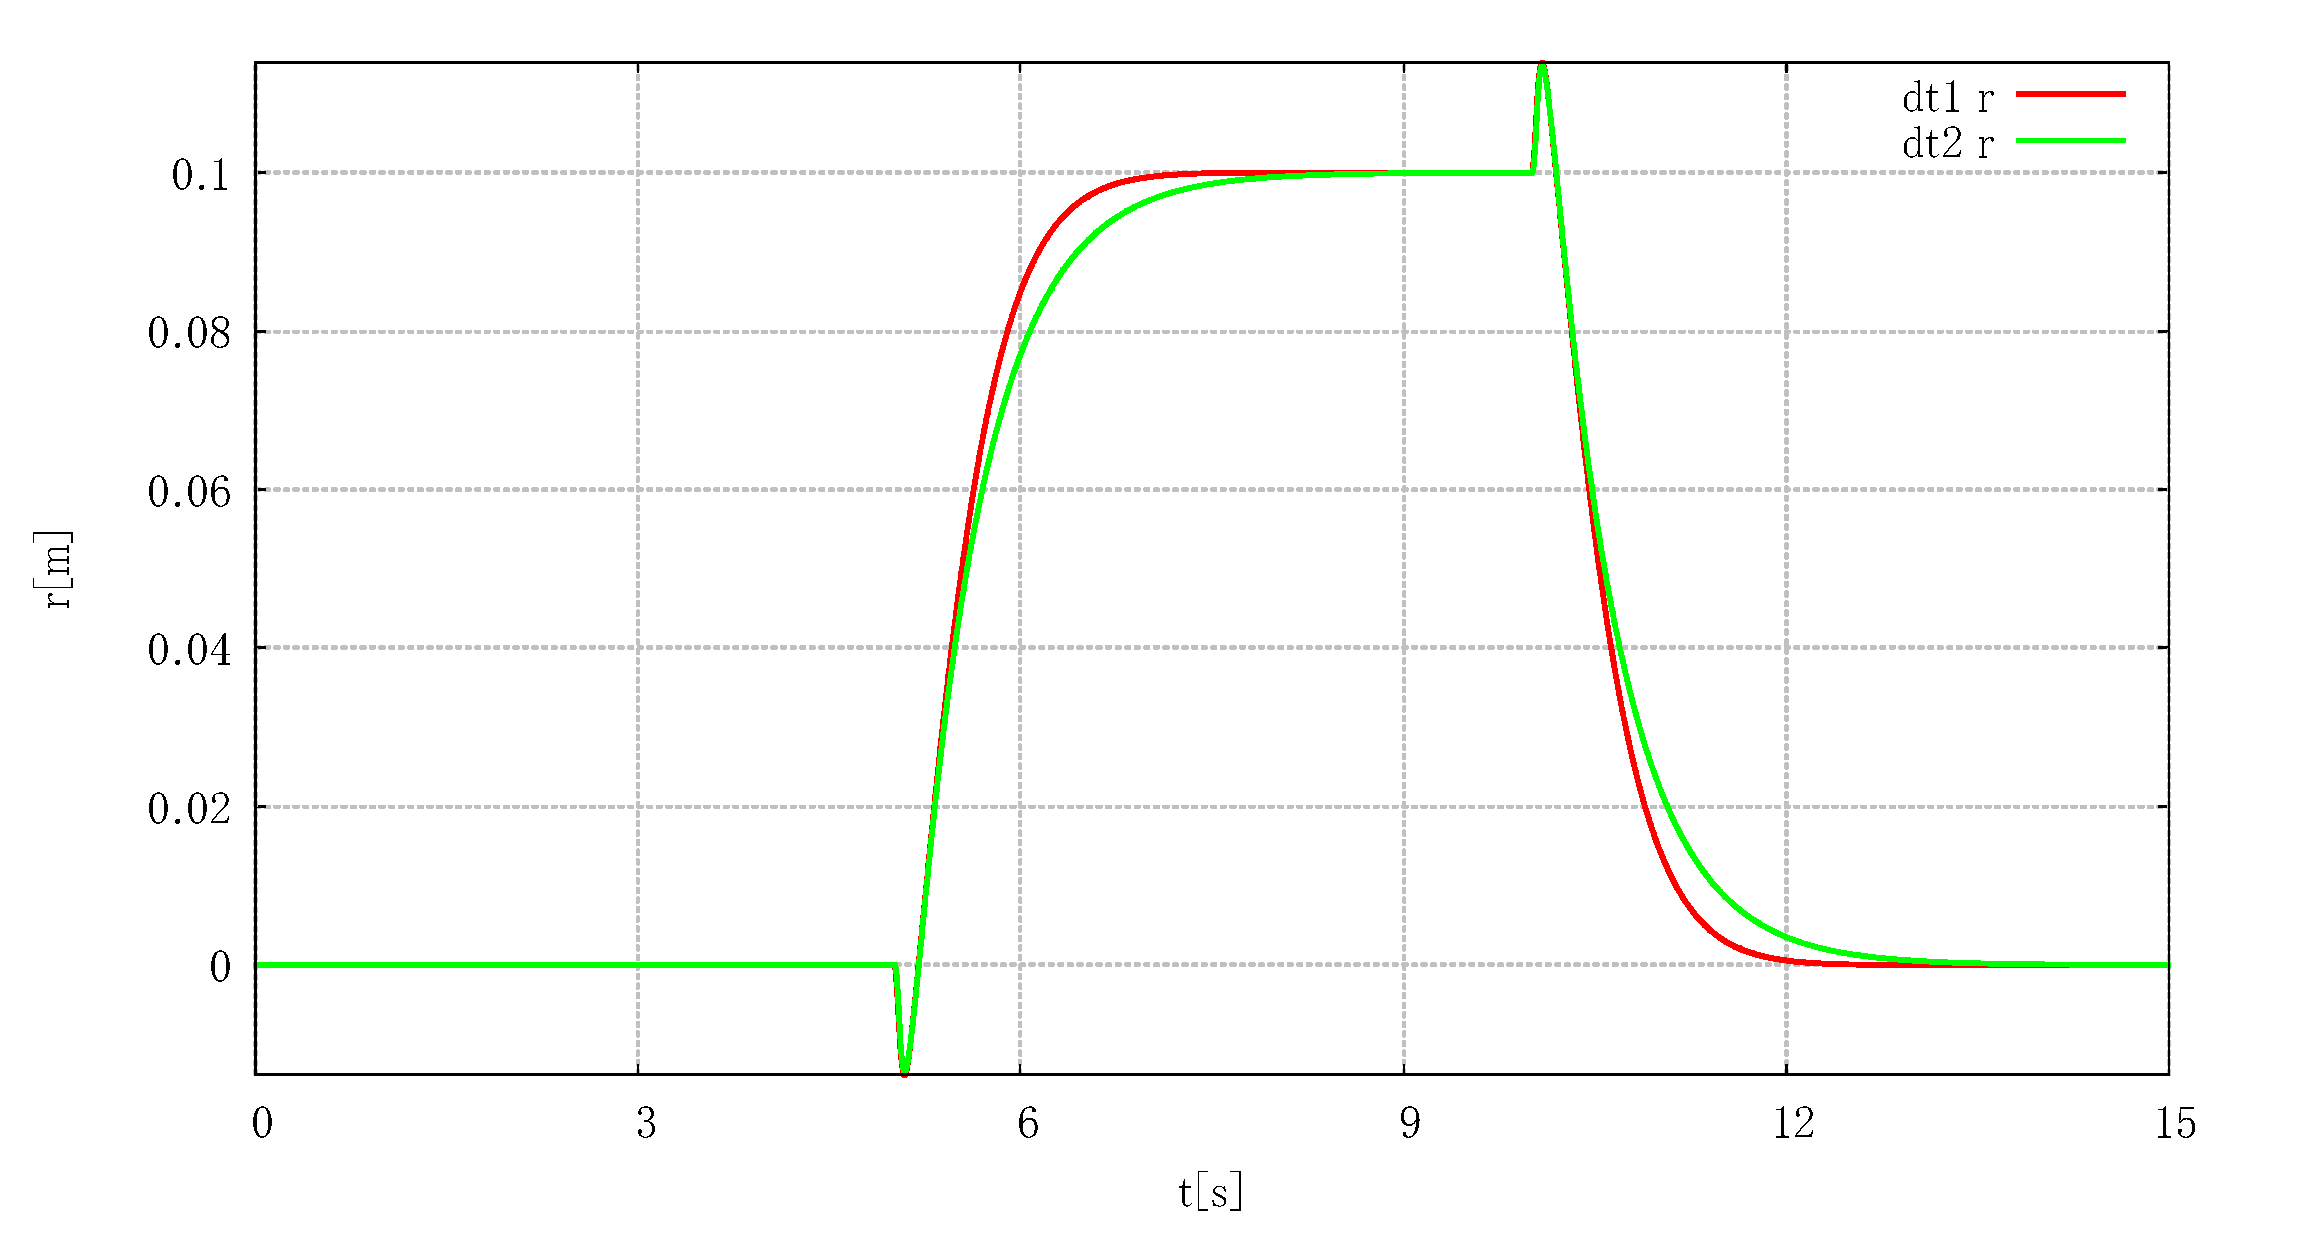
\includegraphics[width=0.8\linewidth]{gazo/simulation_dt_compare_R.eps}
		\caption{サンプリング周期での比較結果(台車位置)}
		\label{image:simulation_dt_r}
	\end{figure}
	\begin{figure}[H]
		\centering
		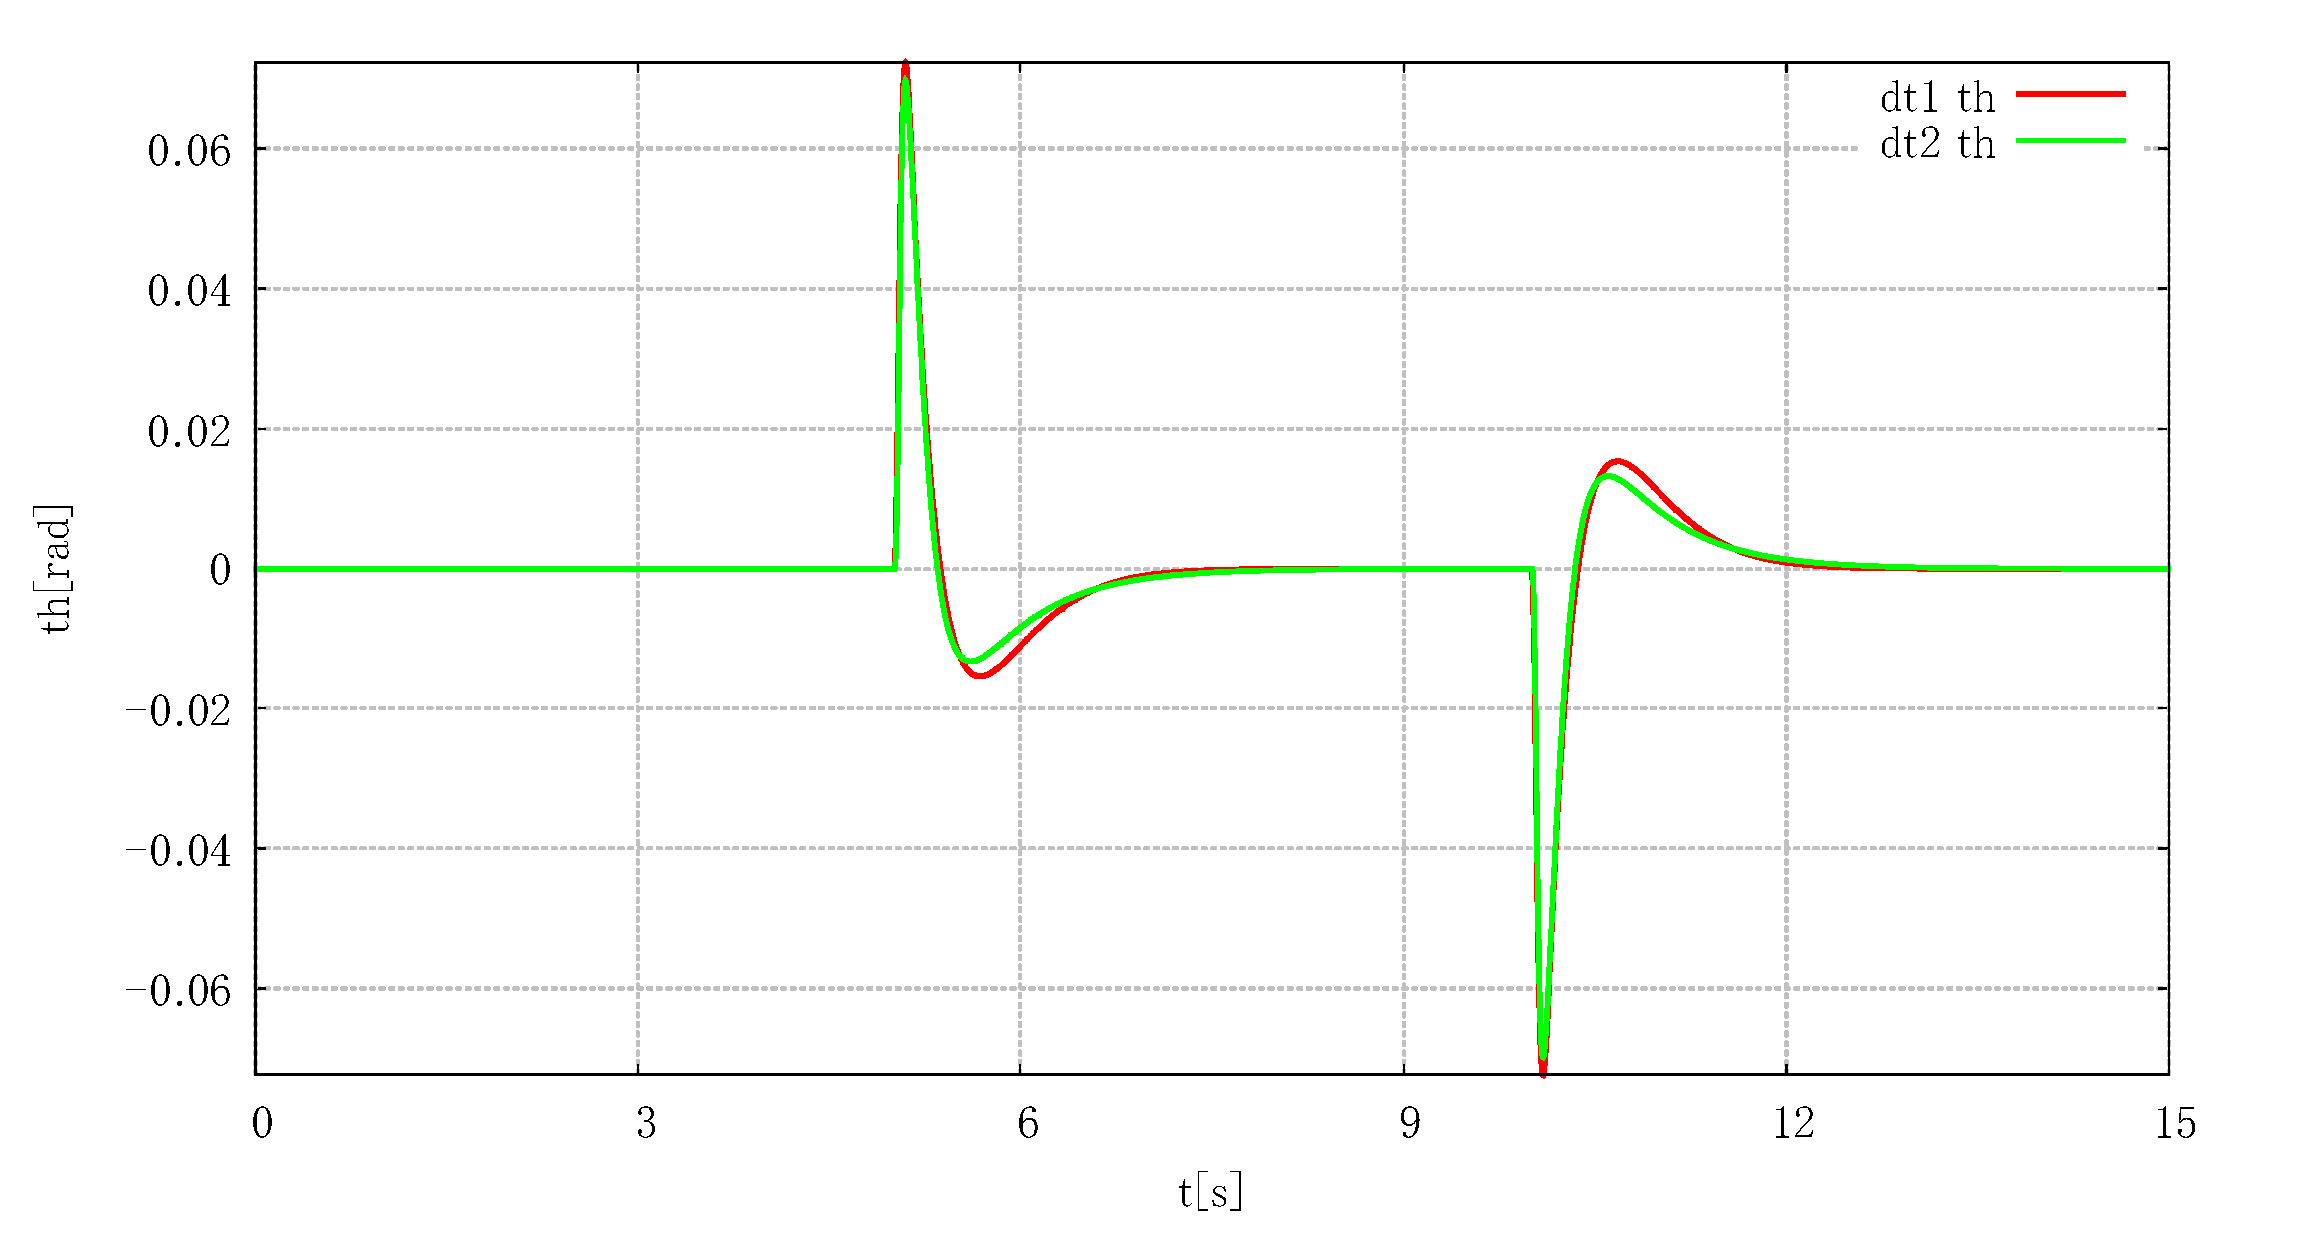
\includegraphics[width=0.8\linewidth]{gazo/simulation_dt_compare_THETA.eps}
		\caption{サンプリング周期での比較結果(振子角度)}
		\label{image:simulation_dt_theta}
	\end{figure}
	図\ref{image:simulation_dt_r}から、パターン1のほうが若干応答が早いといえる。しかし、
	図\ref{image:simulation_dt_r}と図\ref{image:simulation_dt_theta}からは大きな違いを確認することはできない。
	先ほどと同様に倒立振子の状態$x(t)$とオブザーバで推定した値$\hat{x}[k・T]$との差である推定誤差($x(t)-\hat{x}[k・T]$)の応答波形からサンプリング周期の違いによる考察をする。
	以下に台車の速度と振り子の角速度の推定誤差の図を示す。
	\begin{figure}[H]
		\centering
		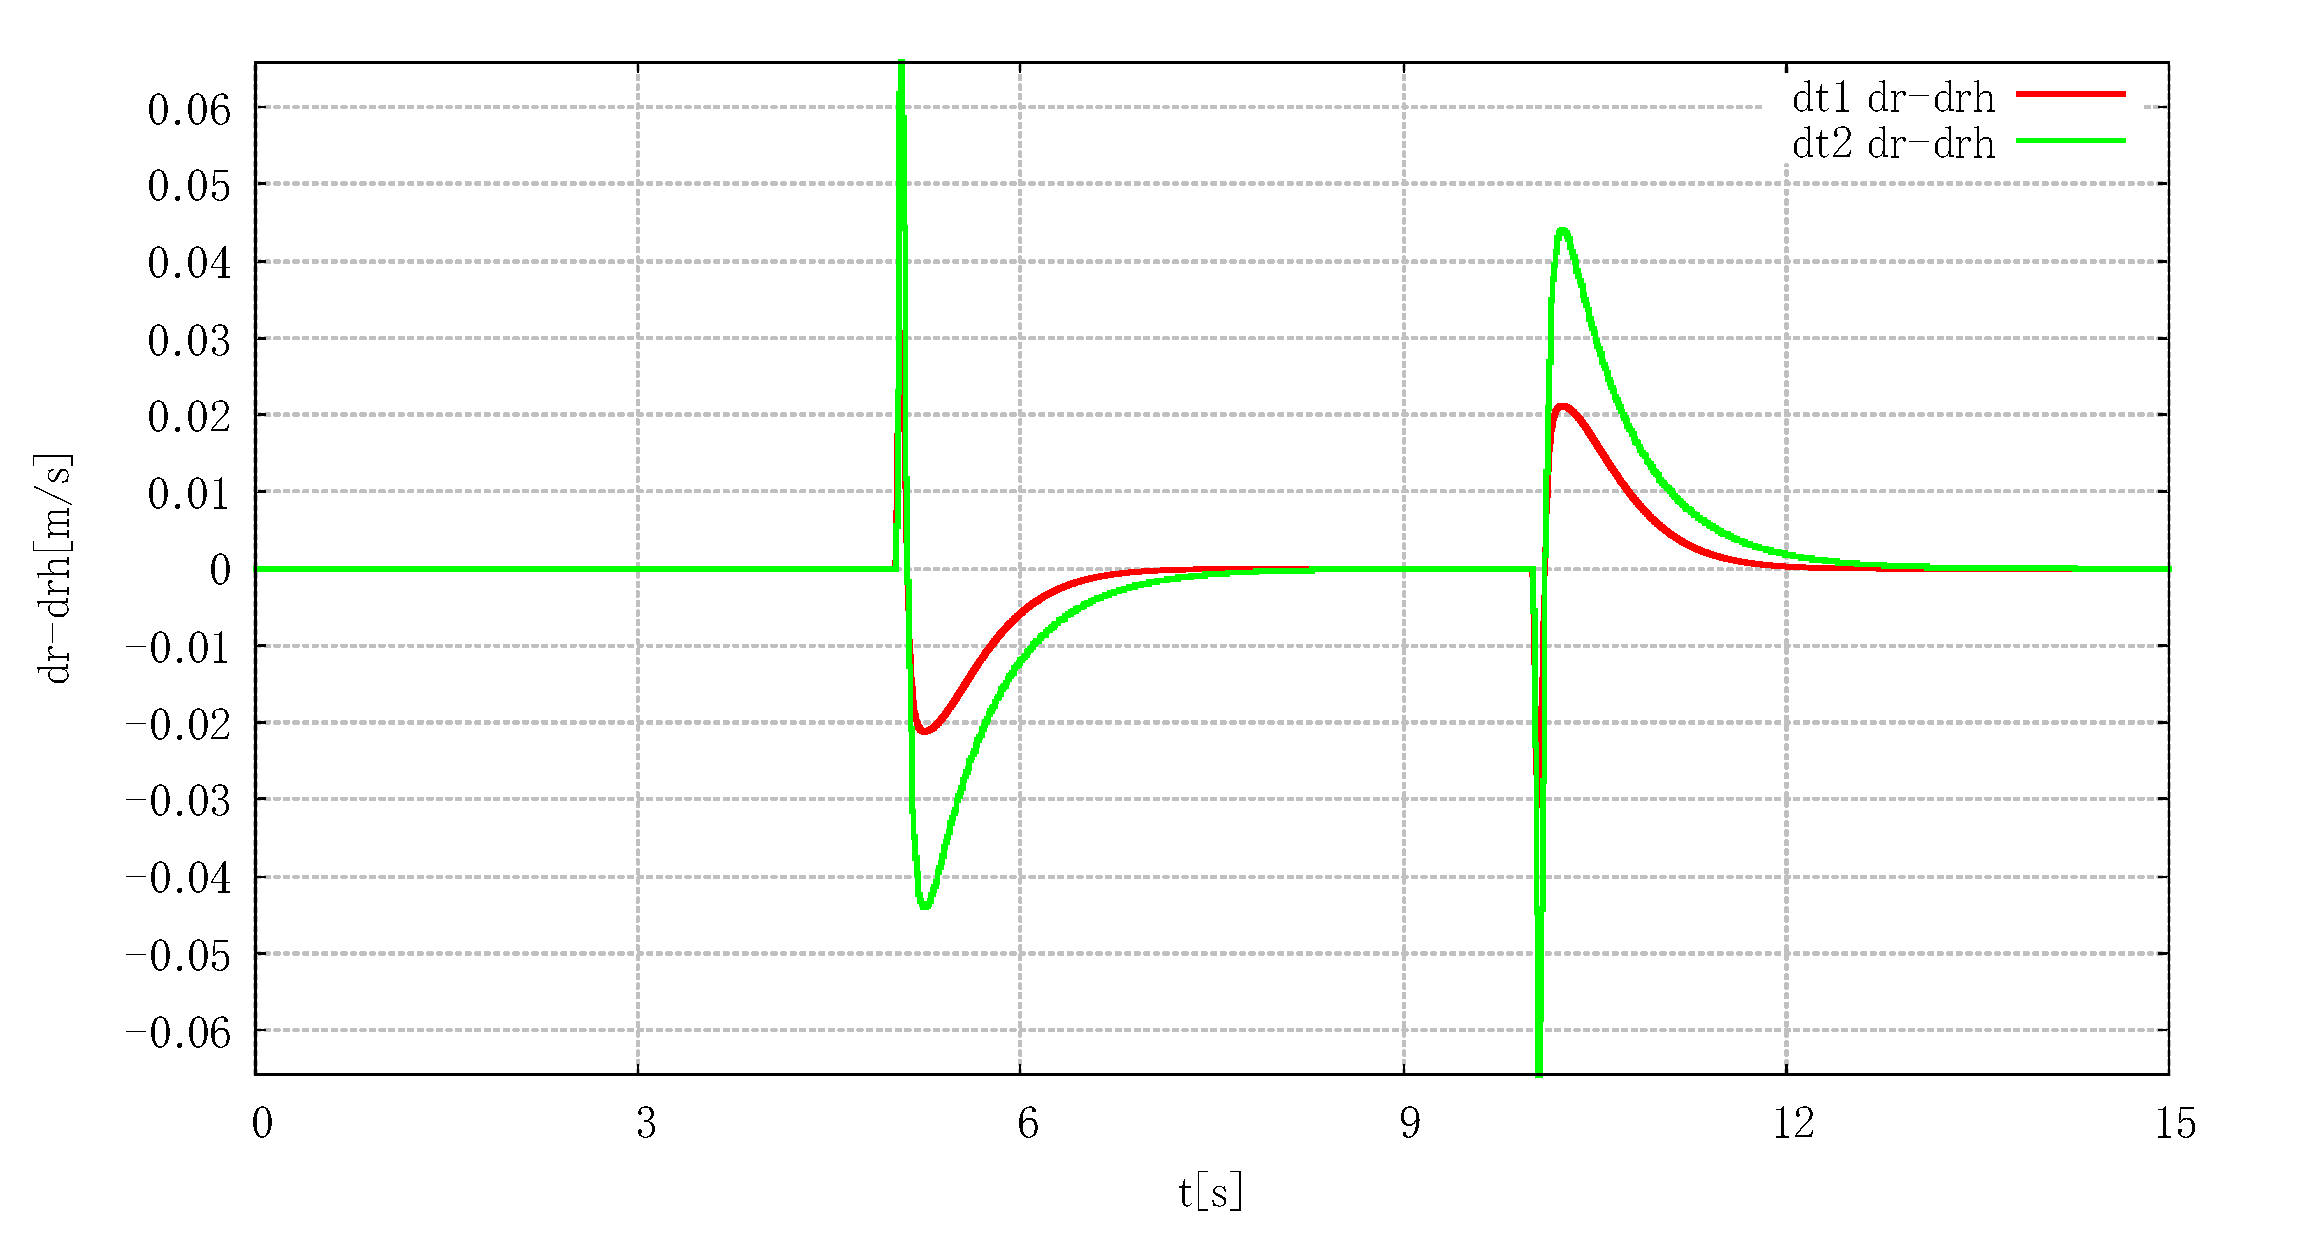
\includegraphics[width=0.8\linewidth]{gazo/simulation_dt_compare_RminusRH.eps}
		\caption{サンプリング周期での推定誤差の比較(台車の速度)}
		\label{image:simulation_dt_rminusrh}
	\end{figure}
	\begin{figure}[H]
		\centering
		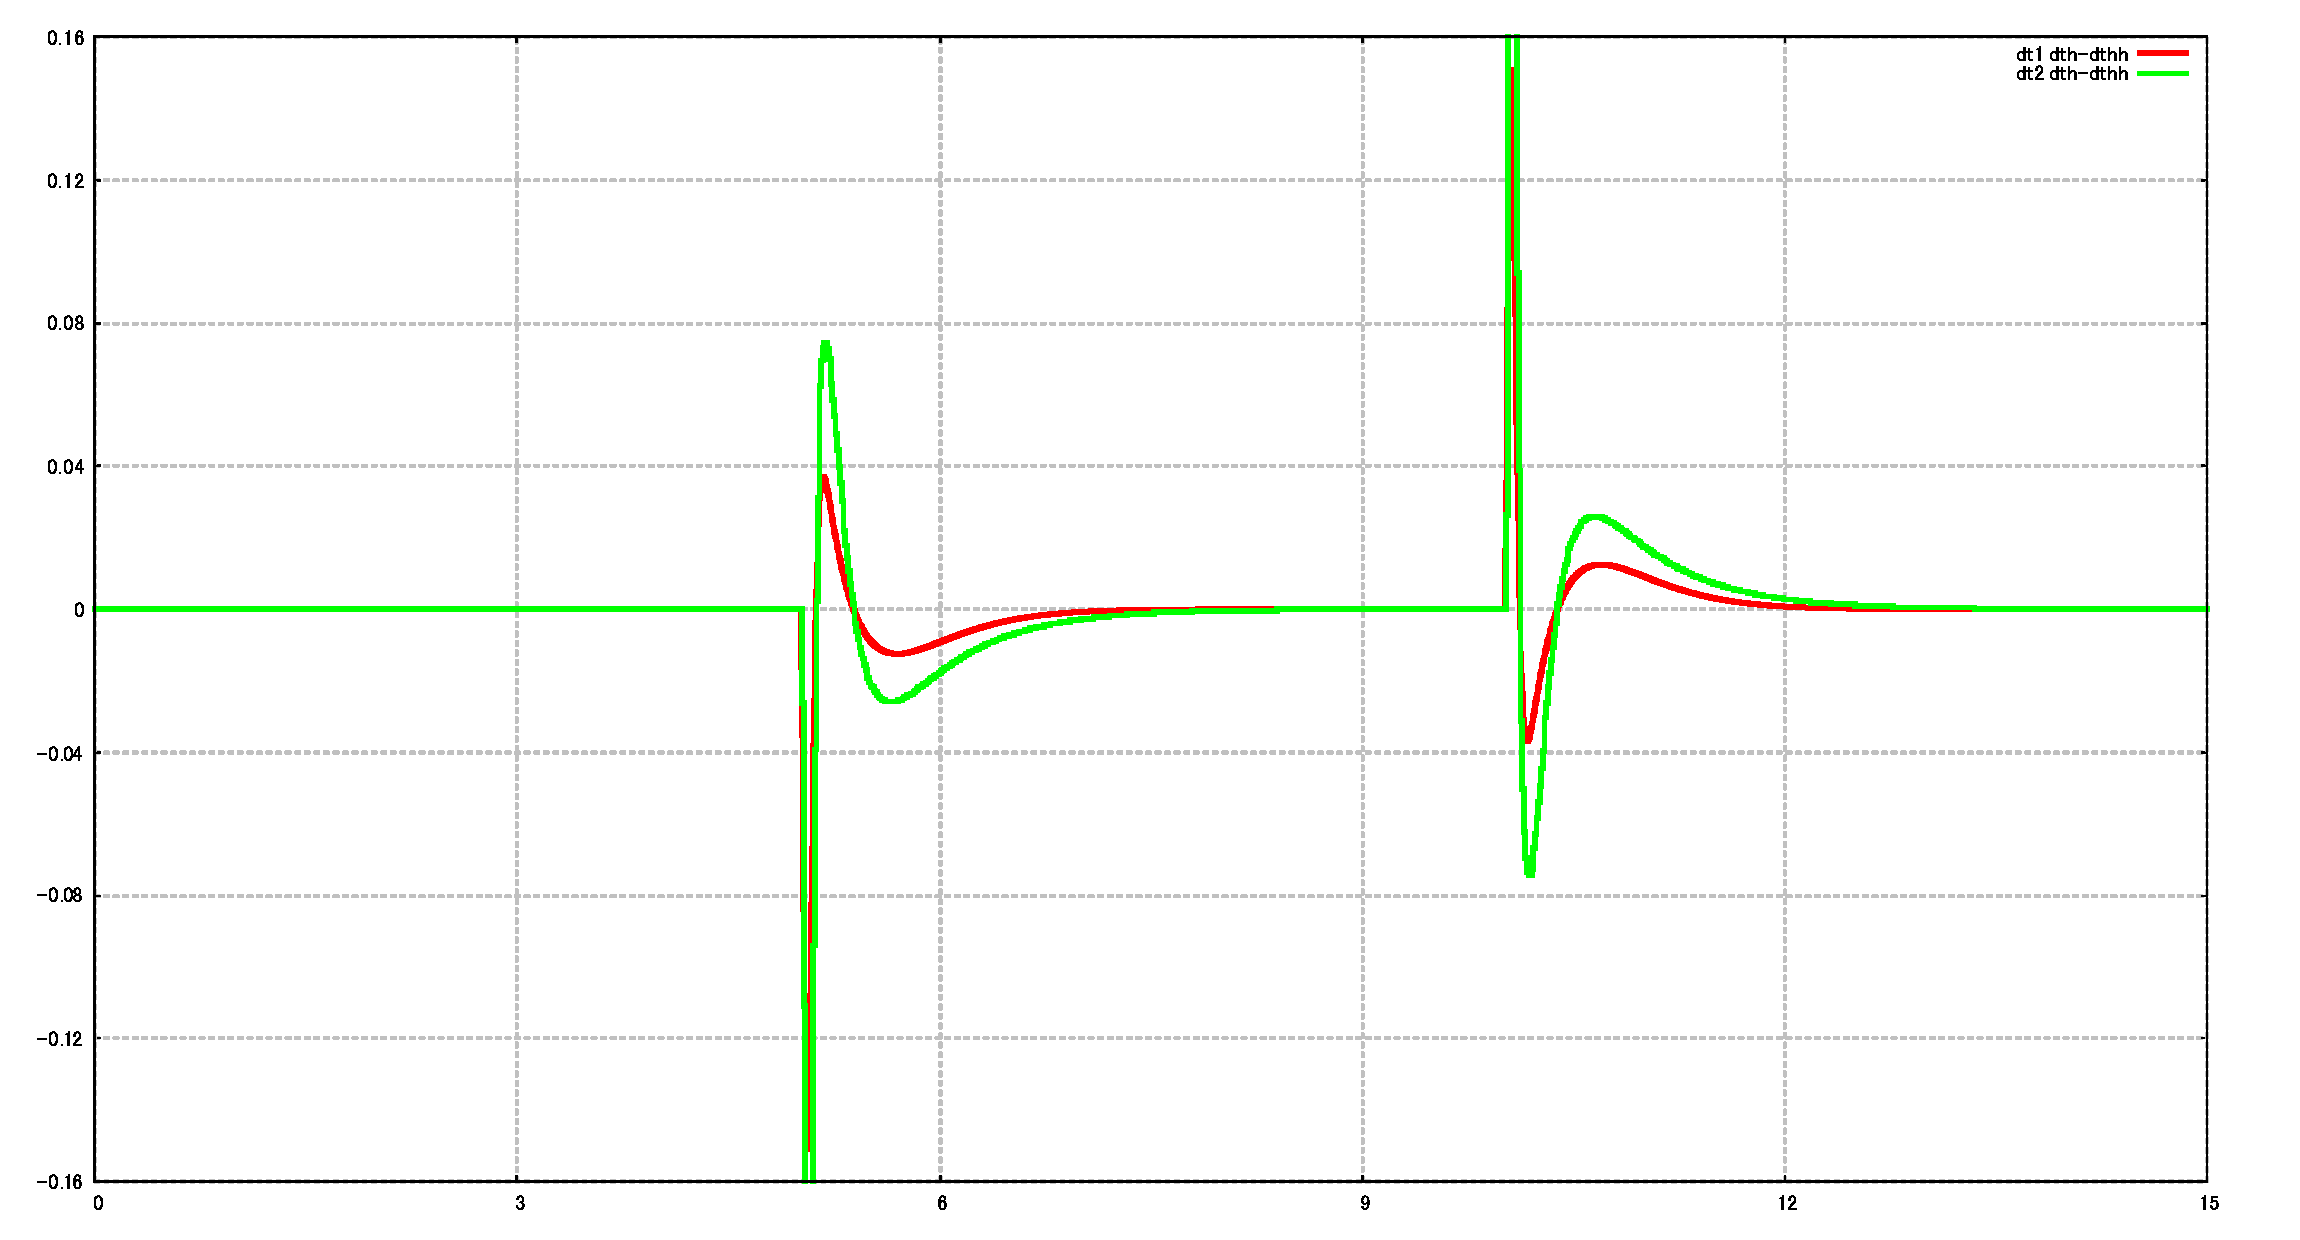
\includegraphics[width=0.8\linewidth]{gazo/simulation_dt_compare_THETAminusTHETAH.eps}
		\caption{サンプリング周期での推定誤差の比較(振子の角速度)}
		\label{image:simulation_dt_thetaminusthetah}
	\end{figure}
	図\ref{image:simulation_dt_rminusrh}と図\ref{image:simulation_dt_thetaminusthetah}よりサンプリング周期の短いほうが
	推定誤差が小さいことが確認できる。
	\par
	以上からサンプリング周期の調整については以下のことが言える。
	\begin{itemize}
	  \item サンプリング周期は短いほうが推定誤差が小さくなり、応答がよくなる。
	  \item ただし、あまり小さくしすぎるのはよくない。
	\end{itemize}
	
%--------------------------------------------------------------------------------------
\section{振り上げ制御及び安定化に対する制御性能評価}
	前節までにおいて、安定化制御における有効なパラメータを考察してきた。
	ここでは、振り上げ制御におけるパラメータ$k,n$を調整することで振り上げ制御の制御性能を考察する。
	\par
	この時、安定化制御に用いるパラメータは以下の表の通りである。
	安定化制御の際に使用するパラメータについてはこれまでの考察に基づいて決定した。
	\begin{table}[H]
		\begin{center}
			\caption{振り上げ後の安定化制御の際に用いるパラメータの組}
			\medskip
			
			\begin{tabular}{|c|c|c|c|}\hline
				重み行列$Q$ & オブザーバの極$P$ & サンプリング周期$\Delta[\rm{s}]$ \\ \hline\hline
				$Q_1$:$\rm{diag}(1E5,1E5,1,1)$ & $P_1$:$((-30,0),(-30,0))^{'}$ & $\Delta_1$:0.005 \\ \hline
			\end{tabular}
		\end{center}
		\label{table:huriage_control}
	\end{table}
	振り上げ制御に用いる各パターンのパラメータは以下の表の通りである。
	\begin{table}[H]
		\begin{center}
			\caption{振り上げ制御に用いるパラメータの組}
			\medskip
			
			\begin{tabular}{|c|c|c|}\hline
				& $n$ & $k$ \\ \hline\hline
				パターン1 & 0.4 & $1.0×10^3$  \\ \hline
				パターン2 & 0.4 & $1.0×10^4$  \\ \hline
				パターン3 & 0.4 & $1.0×10^5$  \\ \hline
			\end{tabular}
		\end{center}
		\label{table:huriage_huriage}
	\end{table}
	以上の表のパラメータを用いて行ったシミュレーションの結果を示す。
	\begin{figure}[H]
		\centering
		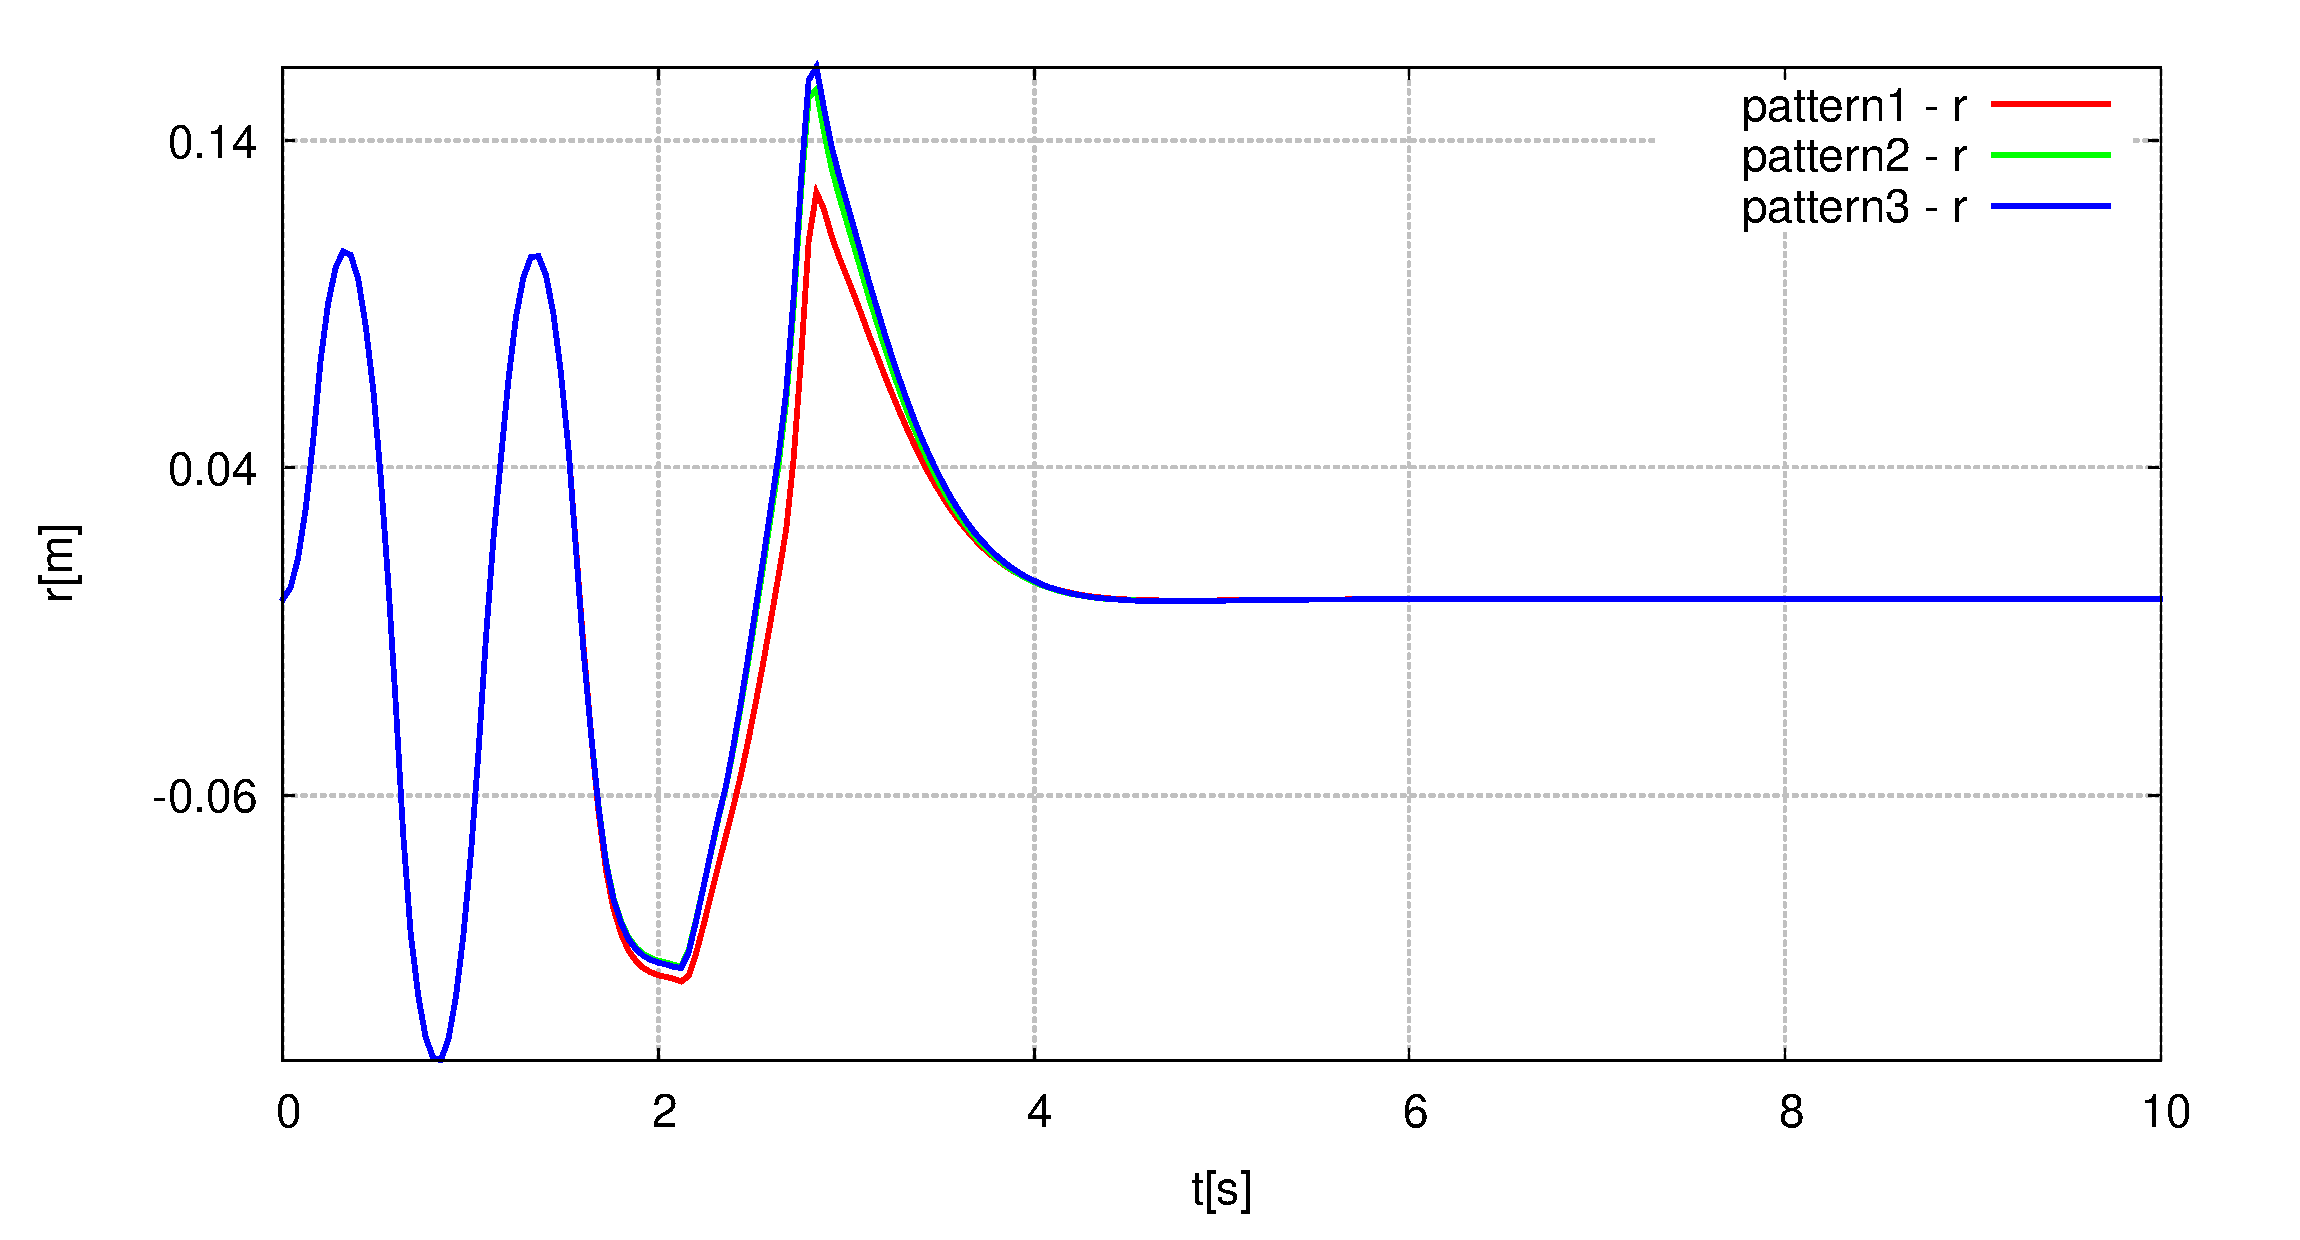
\includegraphics[width=0.8\linewidth]{gazo/Hsimu_R.eps}
		\caption{振り上げ制御のシミュレーション比較結果(台車の位置)}
		\label{image:simu_huriageR}
	\end{figure}
	\begin{figure}[H]
		\centering
		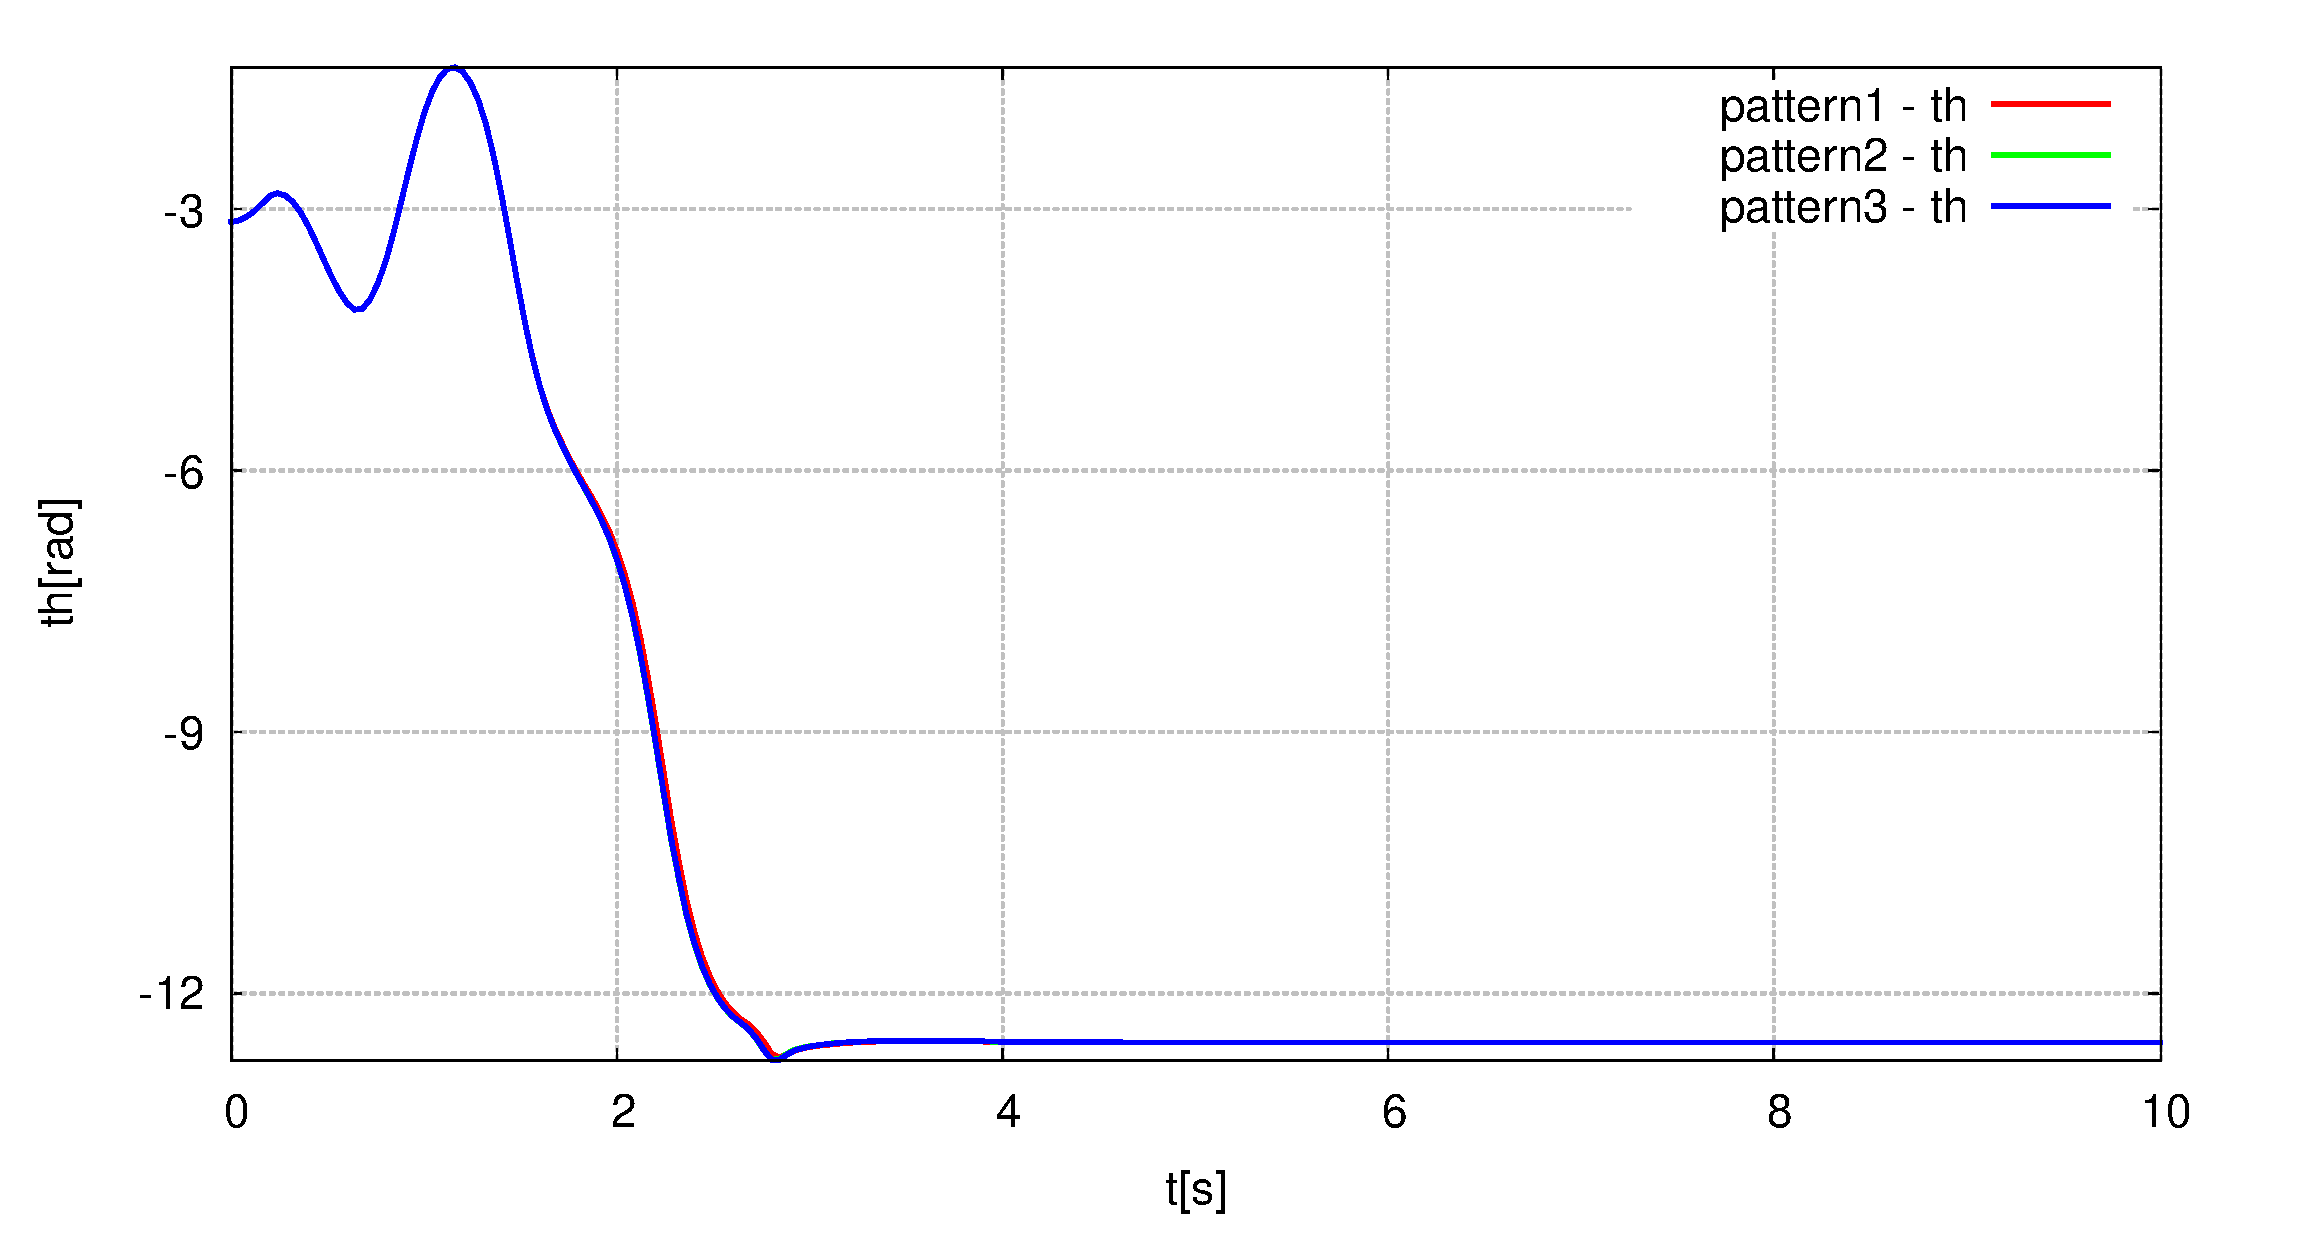
\includegraphics[width=0.8\linewidth]{gazo/Hsimu_TH.eps}
		\caption{振り上げ制御のシミュレーション比較結果(振子の角度)}
		\label{image:simu_huriageTH}
	\end{figure}
	図\ref{image:simu_huriageR}と図\ref{image:simu_huriageTH}よりパラメータ$k$を変えても振り上げ制御から安定化制御に移行するまでの時間に変化がないことがわかる。
	前章のシステム解析においては$k$を大きくすると、エネルギーの収束が早くなると述べた。それにより、振り上げ制御にかかる時間は$k$を大きく
	することで短くなると予想したがそうではなかったようである。
	図\ref{image:simu_huriageR}より、台車の位置に関しては$k$の値によって若干の差異が確認できるが、有意な違いは出ていない。
	図\ref{image:simu_huriageTH}より、振子の角度に関しては$k$の値による差異はほとんど確認できない。
	以上から振り上げ制御に関して以下のことが言える。
	\begin{itemize}
	  \item $k$の値にかかわらず振り上げ制御から安定化制御に移行するまでの時間は一定である。
	  \item $k$の値にかかわらず安定化制御までの台車の位置と振子の角度はほぼ同じ挙動を示す。
	\end{itemize}
	ちなみに、図\ref{image:simu_huriageTH}より、振子の角度が$-12$より小さい値で収束していることから、このシミュレーションでは、
	振子は一回転半してから安定化制御に移ったと考えられる。
	
	
	
%--------------------------------------------------------------------------------------